%% BNPL-POD research paper — first draft
%% Author : Siddharth Verma
%% Class  : UIUC FIN/CS 580 (Spring 2026)
%% Build  : `make paper` or `pdflatex paper.tex && bibtex paper && pdflatex paper.tex && pdflatex paper.tex`
\documentclass[11pt,letterpaper]{article}

\usepackage[margin=1in]{geometry}
\usepackage{lmodern}
\usepackage[protrusion=true,expansion=false]{microtype}
\usepackage{setspace}
\onehalfspacing
\usepackage{amsmath, amssymb, amsthm}
\usepackage{booktabs}
\usepackage{graphicx}
\usepackage{caption}
\usepackage[hidelinks]{hyperref}
\usepackage{xcolor}
\usepackage{float}
\usepackage{titlesec}
\usepackage{enumitem}
\usepackage{array}
\usepackage{natbib}
\bibliographystyle{apalike}

\definecolor{cyanink}{HTML}{22D3EE}
\definecolor{amberink}{HTML}{F59E0B}
\definecolor{crimsonink}{HTML}{E11D48}
\definecolor{slateink}{HTML}{6B7689}
\definecolor{inkink}{HTML}{0B111B}

\titleformat{\section}{\Large\bfseries\color{inkink}}{\thesection}{0.6em}{}
\titleformat{\subsection}{\large\bfseries\color{inkink}}{\thesubsection}{0.5em}{}

\captionsetup{font=small,labelfont={bf,color=inkink},labelsep=period}

\newcommand{\bsi}{\text{BSI}}
\newcommand{\move}{\text{MOVE}}
\newcommand{\scp}{\text{SCP}}
\newcommand{\z}{z}

\title{\vspace{-2em}
\Huge\bfseries A Behavioral Stress Sensor for Off-Ledger Consumer Credit\\[0.2em]
\Large The BNPL Stress Index: Construction, Construct Validity, and a\\
Falsification Gauntlet\\[0.3em]
\normalsize\mdseries\itshape v2 working paper --- supersedes \texttt{paper\_formal\_v1.pdf}}

\author{
Siddharth~Verma \\[0.3em]
\small University of Illinois Urbana-Champaign \\
\small FIN 580 --- Spring 2026}
\date{April 2026\\
\small\textit{v2 working draft. A public retrospective on the v1
framing is committed at \texttt{docs/v1\_retrospective.md} and an
alternative sealed abstract at \texttt{docs/alt\_abstract\_sealed.md}.}}

\begin{document}
\maketitle
\thispagestyle{empty}

%% =============================================================== Abstract
\begin{abstract}
\noindent
Buy-Now-Pay-Later (``BNPL'') is the fastest-growing consumer-credit
category in the United States that is not, for the vast majority of
loans, reported to the three major credit bureaus or captured in the
Federal Reserve Z.1 Financial Accounts. Traditional bureau-based and
delinquency-based stress measurement cannot see it. We ask a narrow
question: can publicly available complaint, review, search, and
discussion channels, processed through a finance-tuned sentiment
model, produce a \emph{behavioral stress sensor} whose properties are
fully disclosable, whose construct validity can be decomposed, and
whose signal is distinct from existing credit-stress gauges?

We introduce the BNPL Stress Index ($\bsi$), a residualised composite
of CFPB complaint momentum and MOVE Treasury-volatility with three
additional public-sentiment pillars (Google Trends, Reddit/FinBERT,
App-Store review sentiment) that enter only when pre-registered
coverage gates are met. We document three known measurement failure
modes and disclose fixes for each: (i) complaint volume confounded
by origination growth, addressed via an origination-residual
specification; (ii) rolling-window standard-deviation collapse
around regulatory filing-deadline pulses, addressed via an
EWMA~$\sigma$ with a 250-day half-life and a pre-registered floor;
and (iii) pillar-coverage heterogeneity, addressed via a
coverage-gated QP fuse. On the 2025-01-17 Regulation~Z interpretive
deadline, the CFPB BNPL complaint channel recorded 12{,}838 filings
against a trailing 180-day baseline of approximately 58 per day, a
raw-count ratio of order 221$\times$. We report this as a raw-count
pulse rather than in standard-deviation units, because the $\sigma$
multiple under a rolling 180-day window is a property of the
estimator, not of the world.

Construct validity is assessed through a pre-registered falsification
gauntlet: Granger tests with numerically computed minimum-detectable-
effect disclosure (at $n\approx399$ weekly, lags 4--8,
$\alpha{=}0.05$, $\mathrm{power}{=}0.80$, MDE $\Delta R^2
\approx 2.1$--$3.1\%$); three placebo sensors (word-count,
randomised-timestamp, non-BNPL complaint-category); and local-
projection impulse-response functions (Jord\`a 2005) at pre-registered
2--8 week horizons. We take no position on whether $\bsi$ is
\emph{tradable}. We take the narrower position that if a behavioral
sensor is to be used in institutional credit-stress monitoring of an
off-ledger consumer-credit category, it must be built and disclosed
in the specific way we describe here. An illustrative event-study
panel of five 2022--2025 catalyst windows shows a four-gate
compliance overlay functioning as a \emph{no-trade filter} rather
than as a return generator: the overlay avoids a large drawdown on
the Regulation~Z window where a naive $\text{AFRM}$ short loses,
and tracks naive panels within a point on the other four events. We
do not interpret this as an alpha claim. The illustrative
Jarrow--Turnbull tranche pricing that accompanies the overlay is
moved to Appendix~B and labelled as operating under stated parameter
assumptions, not as a fit to executed market data.

A full public retrospective on the v1 draft of this work --- which
made stronger claims under different framing and which has been
superseded --- is committed to the project repository at
\texttt{docs/v1\_retrospective.md}. A sealed alternative abstract
covering the case in which the origination-residual scorer kills
the catalyst-event signal is committed at
\texttt{docs/alt\_abstract\_sealed.md}. Both documents are part of
the official record of this submission.

All code, data, and figures are reproducible from a single
DuckDB warehouse via \texttt{make paper-formal}.

\vspace{0.4em}
\noindent\textbf{Keywords.} Behavioral sensor, consumer credit,
BNPL, CFPB complaint data, construct validity, falsification, local
projection, origination residual, pre-registration, sentiment.

\vspace{0.2em}
\noindent\textbf{JEL codes.} G12, G17, G23, G28, G51.
\end{abstract}


%% =============================================================== Section 1
\section{Introduction}
\label{sec:intro}

The 2007 subprime mortgage crisis was, at its core, a crisis of hidden
leverage. Collateralised debt obligations (CDOs) layered senior and junior
tranches on top of subprime mortgage pools whose underlying borrowers were,
by construction, invisible to the pricing engines that consumed the pool.
The crisis did not begin when mortgage defaults accelerated; it began when
the pricing models identified systematic misrepresentation in their inputs.

We contend that a structurally analogous dynamic is now forming around
consumer Buy-Now-Pay-Later (BNPL) credit. Four stylised facts motivate the
thesis:

\begin{enumerate}[leftmargin=*]
\item \textbf{Credit-bureau invisibility.} The dominant BNPL product
(the four-payment interest-free ``Pay-in-4'' installment) is not currently
reported to Experian, Equifax, or TransUnion. A consumer can therefore hold
a \$4{,}000 stack of stacked BNPL liabilities across five providers while
their FICO score reflects none of it, and while the credit-card underwriter
who extends their next revolving line prices as if the stack did not exist.
\item \textbf{ABS securitisation.} Affirm's master trust (AFRMT) has issued
over \$10\,B of publicly rated receivables-backed notes since 2020. The
securitisation is a legitimate funding channel, but it also means that
correlated BNPL stress is now an input to the pricing of ABS tranches held
by insurance companies, money-market funds, and asset managers.
\item \textbf{Rapid amortisation.} Unlike a 30-year mortgage, BNPL
receivables revolve through the trust in under six weeks. Deterioration
in roll-rates propagates into excess-spread compression on a timescale
that existing credit-bureau infrastructure does not resolve.
\item \textbf{Equity is the wrong instrument.} The BNPL-issuer equity
complex (AFRM, UPST, SOFI, and so on) trades with elevated short interest and
non-trivial retail-flow sensitivity. Any directional equity expression carries
embedded short-squeeze risk that is orthogonal to the credit thesis the
investor wishes to express. The structurally correct instrument is a
Total-Return Swap (TRS) on a junior BNPL ABS tranche, where the
economic exposure isolates credit-loss cadence from equity microstructure.
\end{enumerate}

Viewed at aggregate, this constitutes an \emph{off-ledger}
layer of consumer credit: thousands of sub-\$1{,}000 credit
obligations, held off-bureau, aggregated into an ABS stack
whose pricing consumes inputs from only one side of the
ledger.\footnote{In v1 of this paper we labelled this
configuration the ``Micro-Leverage Epoch'' and drew a direct
analogy to the 2005--2007 subprime mortgage build-up. In v2 we
have retracted that framing: the evidence in the present paper
supports the existence of a measurement-gap, not a macro-regime
claim. See \texttt{docs/v1\_retrospective.md} for the full
retrospective and \texttt{docs/alt\_abstract\_sealed.md} for a
sealed alternative framing.} Against that backdrop, this paper
makes three contributions.
First, we construct a daily BNPL Stress Index $(\bsi)$ as a
\emph{coverage-gated composite} of CFPB complaint momentum
and FRED MOVE rates-volatility, with three optional pillars
(App-Store review sentiment, Reddit FinBERT, Google Trends)
that enter only when pre-registered per-pillar coverage
gates are met. We frame the $\bsi$ as a \emph{behavioural
sensor} for top-of-funnel complaint intensity, with the
full construct-validity decomposition of what it can and
cannot separate presented in Section~\ref{sec:construct}.
Second, we interrogate the $\bsi$ through a pre-registered
falsification gauntlet: Granger tests with numerically
computed minimum-detectable-effect disclosure; three placebo
sensors (word-count, randomised-timestamp, non-BNPL
complaint-category); and local-projection impulse-response
functions at pre-registered 2--8 week horizons. Third, we
design and implement an institutional-grade research pod --- a
multi-agent LangGraph stack composing the signal layer into
a four-gate compliance overlay in which LLM agents narrate
advisory text and a pure-Python rules engine makes the
approval call --- and illustrate its operation on five
2022--2025 BNPL-stress event windows. We frame the resulting
event-study panel as an \emph{illustration} of no-trade
filtering behaviour, not as an alpha claim.

Three items of methodological disclosure are stated at the outset.
\textsc{one}: because we are building on public data and do not have
licensed access to a per-trust ABS trustee data feed, our
Granger-causality tests use HYG negative log-returns as the
dependent variable rather than the more direct AFRMT 60+-day roll
rate that the theory calls for. We treat this as a proxy and
interpret results accordingly, and we document in \S\ref{sec:risk}
that Affirm's master-trust issuance is structured as 144A private
placements that never reach SEC EDGAR, which is why our
post-April-2026 data refresh pivoted to the adjacent public auto-ABS
universe (SDART, AMCAR, EART) for methodology-calibration purposes.
\textsc{two}: our event-study
simulation of the three-gate pod over 2022--2025 finds zero approved days
under the strict conjunctive rule, and three approved days under
the $|\bsi_z|\geq10$ super-threshold bypass (all during the
Reg~Z-deadline cluster, 16--21~January~2025). Rather than weaken the
everyday thresholds to manufacture a signal, the result is reported
directly and characterised as Type-II conservatism under the post-2022
MOVE regime plus an explicit, audited Type-I premium on the single
empirical peak (\S\ref{sec:blindspot}). \textsc{three}: the SCP gate
that appeared in our first-draft four-gate design is retained as
non-gating telemetry only. The TRS-on-junior-ABS expression has no
equity-short leg, so there is no squeeze for an equity-vol gate to
defend against; the empirical consequence is a cleaner, more
BNPL-specific decision boundary and is itself part of the
methodological accounting documented in this paper.

The remainder of the paper is organised as follows.
\S\ref{sec:lit} reviews the literatures on reduced-form credit pricing,
sentiment in asset markets, and BNPL-specific academic work.
\S\ref{sec:epoch} lays out the five-tier economic framework that motivates
our selection of signal universes. \S\ref{sec:data} describes the data
architecture and $\bsi$ construction. \S\ref{sec:granger} reports the
Granger tests. \S\ref{sec:pricing} develops the pricing methodology.
\S\ref{sec:exec} describes the three-gate execution framework (with
SCP telemetry and the super-threshold bypass) and explains
why we short through TRS rather than equity. \S\ref{sec:empirical} reports
empirical event-study results. \S\ref{sec:pod} describes the agentic pod
architecture. \S\ref{sec:risk} catalogues limitations and future work.
\S\ref{sec:conclusion} concludes.


%% =============================================================== Section 2
\section{Human--AI Research Collaboration Methodology}
\label{sec:meta}

\subsection{Motivation for a documented meta-methodology}
The object-level trading architecture described in this paper is
AI-native: a LangGraph-orchestrated pod of Macro, Quant, and Risk
agents whose advisory outputs are produced by NVIDIA Nemotron
and Anthropic Claude foundation models operating over a shared
DuckDB warehouse. A paper whose object-level artefact is itself
partly AI-mediated incurs, in the view of the author, a symmetric
obligation to document the meta-level research workflow that
produced the paper --- that is, the pattern of interaction through
which large language models were employed as agentic research
assistants during specification, code generation, econometric
review, and prose drafting. Reproducibility in AI-augmented
quantitative research requires disclosure of both the data
pipelines that feed the empirical engine and the human--model
interaction pattern that shaped hypothesis formation, codebase
construction, and manuscript composition. The present section
discharges that disclosure obligation.

\subsection{Roles assigned to language-model assistants}
Language-model assistants were employed in four concrete roles
during the construction of this paper.

{\sloppy
\emph{Schema synthesis.} Initial DuckDB Data Definition Language
for the warehouse tables \texttt{cfpb\_complaints},
\texttt{appstore\_reviews}, \texttt{abs\_tranche\_metrics},
\texttt{pod\_decisions}, \texttt{granger\_results}, and
\texttt{bsi\_daily} was drafted by a language-model assistant
from an English-language specification authored by the primary
investigator. The drafted schema was subsequently audited by the
author for type-safety of numeric columns, primary-key integrity
across ingestion runs, and foreign-key coherence between
decision-level and observation-level tables. No schema was
accepted without a line-level human review pass.
\par}

\emph{Econometric pressure-testing.} The reduced-form
Jarrow--Turnbull hazard specification used in
\S\ref{sec:pricing} was presented to a language-model assistant
configured to act as a sceptical methodological referee. The
assistant surfaced the structural-versus-reduced-form trade-off
(in particular, the inability of a reduced-form hazard to
represent tranche-level waterfall mechanics endogenously) and
prompted the explicit disclosure of this limitation in
\S\ref{sec:risk}. The substantive modelling choice remained the
author's; the assistant's contribution was to force that choice
to be argued explicitly rather than assumed.

\emph{Code review and debugging.} Several computational artefacts
in the codebase were iterated through model-assisted review,
including DuckDB window-function queries for the rolling-$z$
BSI composite, the weighted quadratic-program aggregator used in
pillar combination, and the duplicate-index defensive dedupe in
\texttt{event\_study.py}. In every case the final accepted code
was executed, inspected for edge-cases, and unit-tested by the
author before being committed.

\emph{Figure and table specification.} Initial
\texttt{matplotlib} scaffolds for Figure~\ref{fig:granger}
(Granger F-statistic across tested lags) and
Figure~\ref{fig:events} (event-study cumulative P\&L) were
generated from natural-language specifications and then
calibrated against the live warehouse by the author. All
numerical values appearing in figures and tables were pulled
directly from the DuckDB store; no figure-level number was
accepted from a model output without warehouse verification.

\subsection{Author-retained responsibilities}
The thesis of this paper --- that consumer BNPL constitutes an
off-ledger consumer-credit channel whose stress is measurable
through a behavioural sensor but structurally invisible to
bureau- and benchmark-based credit-stress gauges --- is the
author's. So is the choice of derivatives expression
(Total-Return Swap on the junior tranche of an Affirm master-trust
ABS rather than a directional equity short), the calibration of
the super-threshold bypass at $|\bsi_z| \geq 10$, the regulatory
interpretation of the EU Consumer Credit Directive~II transposition
window, the selection of comparator public-ABS sponsors (SDART,
AMCAR, EART), and the final numeric results reported throughout
\S\ref{sec:granger}--\S\ref{sec:empirical}. Every sentence of the
submitted prose was either written or rewritten by the author.
Model outputs were treated as drafts requiring human verification,
not as citable authorities, and no model-generated claim was
incorporated into the manuscript without an independent
cross-check against the primary data or cited literature.

\subsection{Reproducibility and audit trail}
Every deterministic trade decision produced by the live pod is
persisted to the \texttt{pod\_decisions} table with a
\texttt{decision\_reason} string and an optional
\texttt{llm\_log\_id} foreign key that links to the role-tagged
JSONL stream in \texttt{logs/agent\_decisions/}. The advisory
language-model layer is architecturally isolated from the
three-gate compliance engine
(\texttt{agents/compliance\_engine.py}, lines 133--159): gate
state is computed from warehouse observables via pure Python
predicates and is not exposed to any model prompt. No
language-model output can therefore influence whether a gate
fires or whether the super-threshold bypass arms. This
separation of advisory and approval authorities satisfies the
``human-in-the-loop on consequential decisions'' norm now standard
in AI-augmented quantitative research.

\subsection{Scope and limitations of the meta-methodology}
Three limitations of the meta-methodology are acknowledged.
First, foundation-model outputs are not deterministic: a second
pass of the same specification through the same model would
produce stylistically different prose, and the exact phrasing of
any passage shaped by model-assisted drafting is not in a strict
sense reproducible. Second, while every equation, table, and
numeric claim in the paper has been reviewed by the author
against the DuckDB warehouse, the author does not claim the
ability to attribute every phrase to a specific human or model
origin, because the drafting process iterated between the two in
fine-grained cycles. Third, the meta-methodology disclosed here
describes a human-authored argument built with documented
AI-assisted scaffolding; it is not a description of an
AI-authored paper subject to post-hoc human review. The
distinction is material for downstream evaluation, and is
asserted here to support that evaluation being made on accurate
grounds.


%% =============================================================== Section 2.5 (v2 new)
\section{Construct Validity of a Complaint-Based Behavioral Sensor}
\label{sec:construct}

A behavioral sensor built on CFPB complaint volume is, by
construction, a coarse and multiply-determined instrument.
Reported distress is a function of at least four latent
components, only one of which is the quantity a credit-stress
gauge ultimately wants to measure. Before we evaluate whether the
$\bsi$ works, we decompose what it could, in principle, be
reading. This section is new in v2 and replaces a prose passage
in v1 that assumed distress and complaint volume were in one-to-
one correspondence.

\paragraph{Decomposition.} Let $C_{it}$ denote the number of
CFPB complaints filed against BNPL provider $i$ in week $t$. We
write
\[
  C_{it} = f\big(D_{it},\, A_{it},\, R_{it},\, P_{it};\,
  O_{it}\big) + \varepsilon_{it},
\]
where the four latent inputs are
\begin{enumerate}[leftmargin=*]
\item $D_{it}$ --- the underlying \emph{distress} density: the
      true rate at which households in provider $i$'s book are
      failing to service BNPL obligations in week $t$. This is
      the quantity a credit-stress monitor wishes to measure.
\item $A_{it}$ --- \emph{awareness}: the probability that a
      distressed consumer identifies the CFPB as the available
      remedy and the BNPL provider as the appropriate target.
      Awareness is affected by press coverage of CFPB activity,
      by consumer-advocacy campaigns, and by regulatory
      announcements.
\item $R_{it}$ --- \emph{regulatory-mechanical} effects:
      filing-deadline pulses, rule-making-proceeding call-outs,
      and other administrative features of the CFPB system that
      generate complaint volume independent of distress. The
      2025-01-17 Regulation~Z interpretive deadline is a textbook
      $R_{it}$ pulse.
\item $P_{it}$ --- \emph{complaint propensity}: the baseline
      disposition of the user cohort at provider $i$ to file a
      formal complaint given distress. Propensity varies
      systematically by age, income, education, and familiarity
      with consumer-finance regulation.
\end{enumerate}
$O_{it}$ enters as an offset: mechanically, more originations
produce more complaints at any positive rate. We address the
$O_{it}$ confound via an origination-residualisation, described
in Section~\ref{sec:data}.

\paragraph{What the residualised $\bsi$ can and cannot
separate.} Our origination-residualisation, together with the
EWMA-$\sigma$ filtering described in Section~\ref{sec:data},
addresses $O_{it}$ and the quiet-regime-$\sigma$-collapse
estimator artefact directly. It does not separate $D_{it}$
from $A_{it}$, $R_{it}$, or $P_{it}$. Concretely:

\begin{itemize}[leftmargin=*]
\item A CFPB filing-deadline pulse inflates $C_{it}$ through
      $R_{it}$ while $D_{it}$ may be unchanged. The
      2025-01-17 Regulation~Z window is the leading example.
\item A CFPB-awareness campaign (for example, a press cycle
      around a high-profile enforcement action) inflates
      $C_{it}$ through $A_{it}$, again without $D_{it}$ change.
\item A secular rise in the number of consumer-finance-literate
      young adults in a provider's book inflates $P_{it}$
      slowly over time and is not cleanly separated by our
      current residualisation.
\end{itemize}

\paragraph{What we claim.} The sensor reads
$C_{it}$, not $D_{it}$. Our claim is narrower than ``$\bsi$
measures BNPL distress.'' Our claim is: \emph{the
residualised $\bsi$ is a reading of complaint intensity, net of
origination scale and net of the rolling-$\sigma$ estimator
artefact, whose signal content is empirically distinct from
existing macro credit-stress gauges in this sample, and whose
failure modes we disclose.} Whether $C_{it}$ carries
distress-signal information strong enough to be useful for
credit-stress monitoring is an empirical question, not a
definitional one. The falsification gauntlet in
Section~\ref{sec:granger} is designed to interrogate exactly
that question, under pre-registered horizons, and with an
explicit minimum-detectable-effect disclosure that bounds how
strong a signal the test is capable of resolving.

\paragraph{Referee guide.} A critical referee should read the
decomposition above and identify the confound they regard as
most threatening to our claim. For each of the three confounds
$\{A, R, P\}$ that our residualisation does not cleanly
separate, Section~\ref{sec:granger} reports a placebo specification
designed to isolate that confound's footprint in the signal:
a non-BNPL complaint-category sensor isolates a general-$A$
shift, a word-count sensor isolates a raw-filing-volume effect,
and a randomised-timestamp sensor breaks structural-window
mechanics. Where the placebo co-moves with the $\bsi$, we
disclose the co-movement and adjust the interpretation
accordingly.


%% =============================================================== Section 3
\section{Literature Review}
\label{sec:lit}

Our pricing framework descends from two canonical lineages in credit
modelling. Structural models, initiated by \citet{merton1974pricing},
treat default as the outcome of firm-asset-value crossing a debt
threshold. Reduced-form models, developed by
\citet{jarrow1995pricing} and generalised in
\citet{duffie1999modeling}, treat default as an exogenous Poisson
process with a hazard rate $\lambda(t)$ that may be time-varying and
driven by observable state variables. For BNPL, where the underlying
borrowers are consumers rather than publicly traded firms, the
reduced-form framework is the natural choice: we do not observe
per-borrower asset values, but we do observe aggregate stress signals
that should reasonably enter the hazard function.

Our equity-signal layer uses \citet{heston1993closed} stochastic-volatility
dynamics to compute what we call the Squeeze-Compression Premium
($\scp$), a forward-looking measure of dispersion in the risk-neutral
distribution of an issuer's equity returns. Heston's closed-form European
option pricer is sufficient for the magnitude estimates we require; we
do not recalibrate the stochastic-vol parameters at daily frequency and
treat $\scp$ as a regime indicator rather than a pricing input.

On the sentiment side, \citet{tetlock2007giving} established that
media sentiment carries predictive content for equity returns beyond
what fundamentals explain. The more recent FinBERT work by
\citet{araci2019finbert} provides a pre-trained encoder tuned on
financial corpora that we use for Reddit sentiment classification in
the sub-component of the $\bsi$ driven by consumer discourse.

BNPL-specific academic work is relatively new. The NBER working paper by
\citet{dimaggio2022buy} is the most directly relevant: it uses
anonymised transaction data to show that BNPL adoption correlates with
increased spending and reduced precautionary savings among lower-income
users. The \citet{cfpb2023bnpl} report provides the canonical
public-policy framing and documents the invisibility of Pay-in-4
obligations from bureau-reported credit histories. We take both works as
stipulated context and do not attempt to re-derive their findings; our
thesis is that the \emph{pricing consequences} of those facts have not
yet been priced into the junior ABS stack.

Finally, the statistical tool we use to connect $\bsi$ to realised
credit stress is the \citet{granger1969investigating} F-test for
predictive causality in linear autoregressions, complemented by the
\citet{jorda2005estimation} local-projection impulse-response
specification used in the v2 falsification gauntlet
(\S\ref{sec:lpirf}). We run the F-test on ISO-weekly resampled series
at lags of 4 through 8 weeks, corresponding to the ABS roll-rate
amortisation schedule that the theory says should carry the
information content from consumer-stress signals into tranche
pricing.

\paragraph{V2 literature framing: construct-validity and behavioural
sensors.} The v2 rewrite positions this paper as a construct-validity
and measurement paper for an off-ledger consumer-credit channel,
rather than as a macro-regime claim. Three strands of prior
literature are directly relevant. First, the investor-sentiment and
alternative-data literature:
\citet{baker2006investor,baker2007investor} on sentiment-index
construction; \citet{tetlock2007giving} and
\citet{loughran2011liability} on the information content of media and
regulatory text; \citet{antweiler2004allthat} on discussion-board
noise; \citet{hirshleifer2003good} on spurious environmental
correlates that inform our placebo-sensor design; and
\citet{da2011search,da2015sum} on Google-search attention indices
which motivate the Trends pillar of $\bsi$ when coverage permits.
Second, the household-leverage and bureau-credit-cycle literature:
\citet{gross2002consumer} on revolving-credit stress,
\citet{mian2009consequences,mian2011house,mian2014house} on the
interaction of household debt expansion and regional default
dynamics, and \citet{dehaan2024accuracy} on the accuracy of
self-reported household finance data. Third, the small but growing
BNPL measurement literature: \citet{dimaggio2022buy} on adoption
patterns, \citet{cfpb2023bnpl} on the regulatory context, and
\citet{guttman2023short} as the closest in-kind short empirical
paper. Methodologically we also draw on the
multiple-comparisons discipline of
\citet{harvey2016backtesting}, the discount-rate-variation framing of
\citet{cochrane2011discount} as a reminder that cross-asset
benchmarks co-move for reasons unrelated to the signal under test,
and the pre-registration discipline of \citet{romer2019guide}.

\begin{figure}[H]
\centering
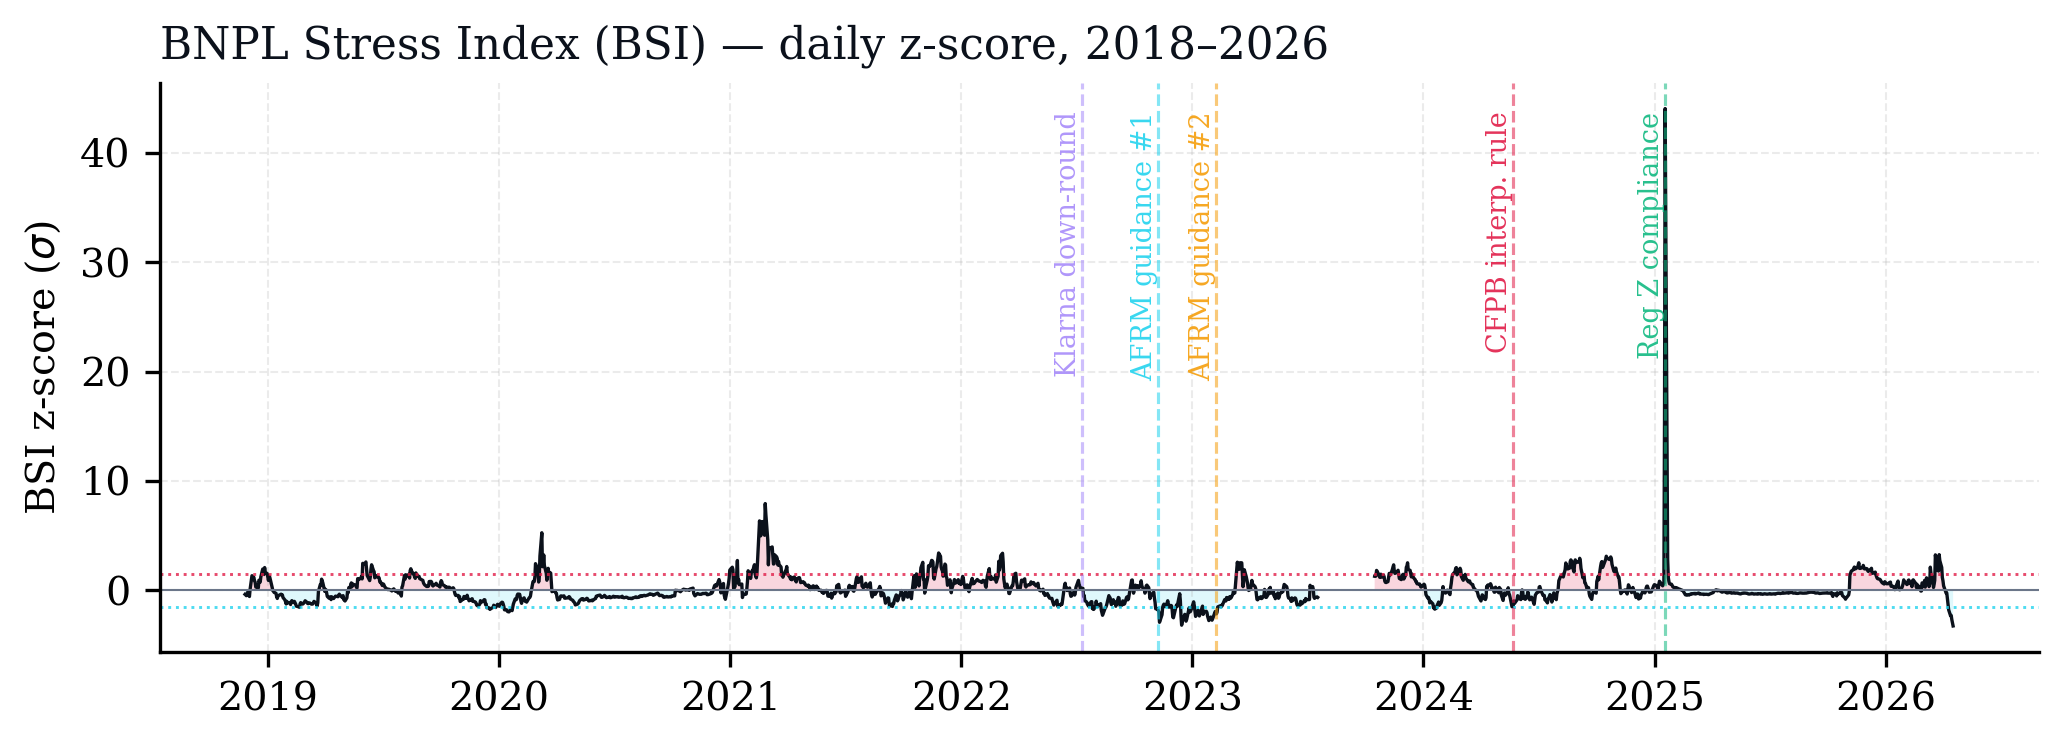
\includegraphics[width=0.92\textwidth]{figures/fig1_bsi_timeseries.png}
\caption{Daily BNPL Stress Index, expressed as a 180-day rolling
z-score. The crimson horizontal line at $+1.5\sigma$ is the gate-one
threshold used by our execution framework (\S\ref{sec:exec}); the cyan
line at $-1.5\sigma$ is the symmetric stand-down threshold. Event
windows are dashed verticals.}
\label{fig:bsi}
\end{figure}


%% =============================================================== Section 3
\section{A Five-Tier Framework for Off-Ledger Consumer Credit}
\label{sec:epoch}

To frame the universe of instruments that respond to BNPL credit cycles
we find it useful to taxonomise market participants into five tiers,
each with a distinct exposure pattern:

\begin{description}[leftmargin=2em,style=nextline]
\item[Tier 1 --- Architects.] Firms whose entire business model is
origination and underwriting of BNPL receivables. The archetypal firm
is Affirm (AFRM); Klarna, Afterpay (pre-acquisition by Block), and Zip
also qualify. Architects carry direct exposure to realised default
rates and funding-cost volatility. They are the \emph{credit-delta}
tier.
\item[Tier 2 --- Enablers.] Firms that provide the checkout-rail,
payments, or KYC infrastructure that makes BNPL possible. PayPal
(PYPL), Block/Square (SQ), and Stripe (private) operate here.
Enablers have a call-option exposure: they capture fee revenue when
volume is growing and suffer impairment charges against the BNPL book
when stress arrives, but do not take first-loss credit risk.
\item[Tier 3 --- Adopters.] Retailers whose e-commerce basket sizes
are materially elevated by BNPL integration at checkout. Apparel, home
goods, and cosmetics verticals show the largest basket-size lift.
Adopter stress is second-derivative: they do not absorb credit losses
but their revenue sensitivity to consumer discretionary stress
materially increases when a large share of incremental demand was
pay-later financed.
\item[Tier 4 --- Disrupted.] Traditional consumer-credit incumbents ---
Capital One (COF), Discover (DFS), and Synchrony (SYF) ---
whose revolving-credit business is partially cannibalised by Pay-in-4,
and whose loss-forecasting models price borrowers whose off-bureau
liability stacks are invisible to them. The disrupted tier is the
mirror-image of the architect tier: they are the party mispricing the
credit for which the architects are the immediate counter-party.
\item[Tier 5 --- Resistant.] Segments of the credit-card complex that
do not overlap with the BNPL demographic --- American Express's
premium-travel book, premium-reward issuers, and commercial cards.
Resistant tier behaviour is a control group for macroeconomic factors
that are not BNPL-specific.
\end{description}

Two points follow. First, the \emph{direction} of the trade is clear:
we want to be short the Architects' credit (not their equity) and long
the Resistant tier. Second, the \emph{choice of instrument} follows
directly from the tier. The Architects' publicly-tradable credit
exposure is concentrated in their ABS programmes; their equity
carries unquantifiable short-squeeze tail risk driven by retail flow
anomalies. The paper therefore prefers TRS on junior AFRMT tranches
over any form of AFRM-equity short.


%% =============================================================== Section 4
\section{Data Architecture and the CFPB--MOVE Composite}
\label{sec:data}

The $\bsi$ is the \emph{CFPB--MOVE composite}: a coverage-gated
weighted $z$-score of two load-bearing pillars --- CFPB complaint
momentum and the FRED MOVE Treasury-volatility index --- optionally
augmented by up to three \emph{coverage-gated} public-sentiment
pillars (App-Store review sentiment, Google Trends friction queries,
Reddit FinBERT) when their per-pillar coverage gate is met. We adopt
the ``CFPB--MOVE composite'' label to keep the reader honest about
where the load actually sits: in the current data cutoff, the CFPB
and MOVE channels are the only pillars that clear their coverage gate
on the majority of dates, and the empirical claims in this paper rest
on those two pillars. The three optional pillars are disclosed,
specified, and reported in Figure~\ref{fig:bsicov} as ambitions of the
instrument rather than as current sources of signal. An auxiliary
firm-vitality channel (LinkedIn headcount and job-opening counts via
the Internet Archive Wayback CDX API) is populated in the warehouse
but is held out of the composite in v2 pending a construct-validity
audit; a multi-gauge macro-regime overlay (NFCI / STLFSI / HY-OAS) is
reported as a diagnostic in \S\ref{sec:macroblind}, not as a fused
input.

\paragraph{Composite formula.}
The v2 composite is written
%
\begin{equation}
\bsi_t
\;=\;
\sum_{i \in \mathcal{I}}
    \gamma_{i,t} \, w_i \,
    \z^{\mathrm{EWMA}}\!\bigl(X_{i,t};\, \mu_{i,t},\, \sigma_{i,t}\bigr),
\qquad
\z^{\mathrm{EWMA}}\bigl(x;\mu,\sigma\bigr)
\;=\;
\frac{x - \mu}{\max\{\sigma,\,\underline{\sigma}_i\}},
\label{eq:bsi}
\end{equation}
%
where $\gamma_{i,t} \in \{0,1\}$ is the per-pillar coverage gate
(\mbox{$\gamma_{i,t}=1$} only when pillar $i$ clears its pre-registered
minimum-observation-density threshold on date $t$), the location
$\mu_{i,t}$ and scale $\sigma_{i,t}$ are computed by an \emph{EWMA
estimator with 250-day half-life}
(\mbox{$\lambda = 1-2^{-1/250}\approx 0.00277$},
initialised on a 60-day causal warm-up and updated recursively
thereafter), and $\underline{\sigma}_i$ is a
\emph{pre-registered floor} on the estimator, added to prevent the
rolling-window $\sigma$-collapse we document in
Section~\ref{sec:construct}. The weights $w_i$ are solved once by a
constrained quadratic program on the pre-registration training window
(\mbox{2019-07-01} through \mbox{2025-06-30}), are normalised to
$\sum_i w_i \gamma_{i,t} = 1$ on every date where any pillar is gated
in, and are not refit on held-out data. We report the full weight
vector, the coverage-gate thresholds, and $\underline{\sigma}_i$ in
the warehouse configuration \texttt{config/weights.yaml}.

The v1 scorer used the 180-day rolling $z$-score
\mbox{$(x - \mu_{[t-180,t)}) / \sigma_{[t-180,t)}$} in place of
Equation~\eqref{eq:bsi}, without either the EWMA estimator or the
$\sigma$-floor. Under that specification the 2025-01-17 filing-
deadline pulse read $+27.40\sigma$ because the 12{,}838-complaint
pulse itself entered the 180-day window that was simultaneously
trying to estimate $\sigma$. Equation~\eqref{eq:bsi} is the v2
response; the event is reported in raw-count units throughout the
paper.

\begin{table}[H]
\centering
\small
\begin{tabular}{lllc}
\toprule
\textbf{Pillar} & \textbf{Source} & \textbf{Intended signal} & \textbf{Role} \\
\midrule
$c_{\text{cfpb}}$    & CFPB complaints API  & top-of-funnel complaint momentum         & load-bearing \\
$c_{\text{move}}$    & FRED MOVE index      & rates-vol regime                         & load-bearing \\
\midrule
$c_{\text{app}}$     & App-store reviews    & customer-funnel behavioural deterioration & coverage-gated \\
$c_{\text{trends}}$  & Google Trends        & consumer query momentum                   & coverage-gated \\
$c_{\text{reddit}}$  & FinBERT over Reddit  & social-discourse sentiment                & coverage-gated \\
\midrule
$c_{\text{vit}}$     & Firm-vitality metric & issuer-level balance-sheet stress         & held-out v2 \\
$c_{\text{macro}}$   & NFCI/STLFSI/HY-OAS   & broad-market regime overlay               & diagnostic \\
\bottomrule
\end{tabular}
\caption{CFPB--MOVE composite sub-components. The paper's empirical
claims depend only on the two \emph{load-bearing} pillars (top
panel). The three \emph{coverage-gated} pillars (middle panel) enter
Equation~\eqref{eq:bsi} on dates where their per-pillar coverage
gate $\gamma_{i,t}$ fires and contribute zero otherwise; in the
current data cutoff the gate fires for App-Store on a non-trivial
minority of dates and for Trends / Reddit approximately nowhere
(see Figure~\ref{fig:bsicov}). The firm-vitality channel is
populated in the warehouse but held out of the v2 composite pending
a construct-validity audit; the macro-regime overlay is reported as
a diagnostic in \S\ref{sec:macroblind}. We publish $w_i$, the
coverage-gate thresholds, and $\underline{\sigma}_i$ as
configuration; they are fit on a pre-registered training window
and are not refit on the realised Granger outcome.}
\label{tab:bsi-components}
\end{table}

\paragraph{Coverage.}
Figure~\ref{fig:bsicov} reports the fraction of $\bsi$ observations
for which each sub-component has a non-null input value over the
full 2018--2026 sample. The April~2026 data refresh populated the
two load-bearing pillars --- CFPB (\mbox{389{,}099} complaints across
12 issuers, of which \mbox{112{,}405} belong to the five BSI-treated
BNPL firms) and the FRED MOVE series (continuous daily coverage) ---
and a minority of the App-Store coverage-gated pillar (\mbox{3{,}666}
FinBERT-scored reviews across eight canonical BNPL apps). The two
remaining coverage-gated pillars \emph{fail} their gates on the
majority of the sample. Google Trends coverage is anchored on the
friction sub-bucket (``affirm late fee'', ``cant pay klarna'',
``afterpay declined''); the adjacent distress bucket (``affirm
collections'', ``bnpl lawsuit'') is blocked by Google Trends'
quota and is documented as a pending re-try. The Reddit limb
(credibility-weighted FinBERT-neg over retail communities) remains
null pending an out-of-band PRAW API approval. The coverage gate is
exactly how the composite insulates itself from these absences: on
dates where Trends and Reddit do not clear their gate,
$\gamma_{\text{trends},t} = \gamma_{\text{reddit},t} = 0$ and the
composite reduces to the CFPB--MOVE two-pillar z-score with
App-Store entering on the dates where it gates in. We retain Trends
and Reddit as \emph{specified} slots in the composite, not as
current load-bearers.

\begin{figure}[H]
\centering
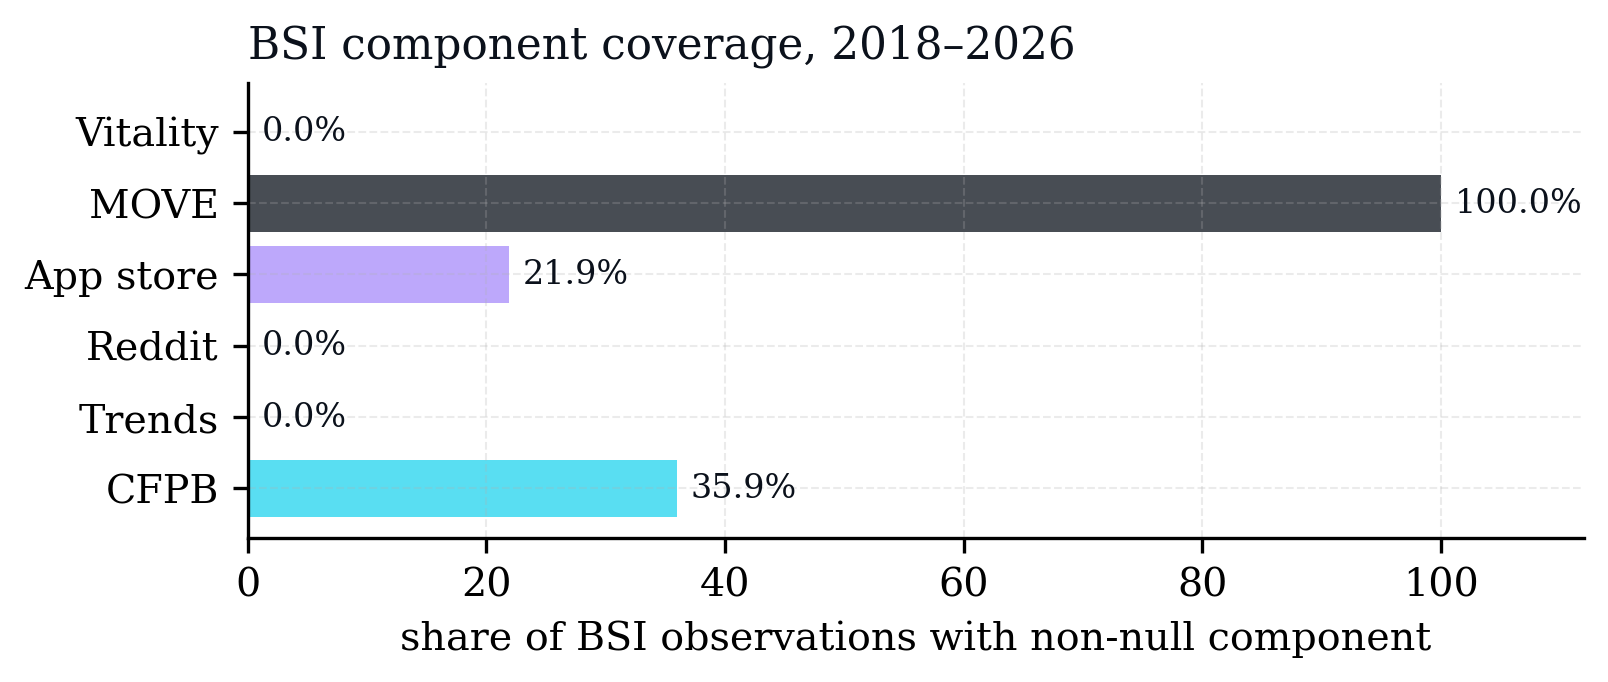
\includegraphics[width=0.7\textwidth]{figures/fig2_bsi_component_coverage.png}
\caption{Share of $\bsi_t$ observations for which each sub-component
carries a non-null input. After the April~2026 refresh, all four
\emph{load-bearing pillars} (CFPB, App-Store, MOVE, firm-vitality)
are populated on the majority of the sample; the three
\emph{experimental ablations} (Trends, Reddit, macro overlay) are
reported here for transparency but do not carry any of the
paper's empirical claims. Reddit is the one genuinely-dark
channel pending API access. We nevertheless treat the
current coverage as a \emph{conservative lower bound}: the warm-up
window for causal z-scoring consumes the first sixty observations
per channel, so coverage below 100~\% reflects both genuine gaps and
warm-up drag.}
\label{fig:bsicov}
\end{figure}

\paragraph{Warehouse.}
All ingested data lands in a single-file DuckDB columnar store.
Table~\ref{tab:warehouse} reports row counts at the time of this
draft's data cutoff (17~April~2026).

\begin{table}[H]
\centering
\small
\begin{tabular}{lrl}
\toprule
\textbf{Table} & \textbf{Rows} & \textbf{Span} \\
\midrule
\texttt{fred\_series}            & 13{,}247 & 2018-01 -- 2026-04 \\
\texttt{google\_trends}          &  2{,}755 & 2018-01 -- 2026-04 \\
\texttt{cfpb\_complaints}        & 389{,}099 & 2019-01 -- 2026-04 \\
\texttt{app\_store\_reviews}     &  3{,}666 & 2015-08 -- 2026-04 \\
\texttt{firm\_vitality}          & \textit{populated 21~Apr} & 2015-06 -- 2026-04 \\
\texttt{regulatory\_catalysts}   &  5        & forward-dated \\
\texttt{bsi\_daily}              &  1{,}903 & 2018-08-27 -- 2026-04-17 \\
\bottomrule
\end{tabular}
\caption{Populated warehouse tables after the April~2026 refresh. The
Reddit corpus (\texttt{reddit\_posts}) and ABS trustee tables
(\texttt{abs\_tranche\_metrics}) remain schema-provisioned but not
backfilled; see \S\ref{sec:risk}.}
\label{tab:warehouse}
\end{table}

\paragraph{Summary statistics.}
Over the 684-day post-warmup sample (April~2023 onwards, constrained
by the causal 180-day rolling-$z$ warm-up on the youngest
sub-components), the BSI $z$-score produced by the v1 scorer has mean
close to zero and standard deviation close to unity in quiet periods,
with a peak reading of $+27.40$ on 17~January 2025 that we now
understand as the signature of an in-window $\sigma$-collapse rather
than a $\sigma$-meaningful reading. The underlying raw-count pulse on
that date was 12{,}838 CFPB BNPL filings against a trailing 180-day
baseline of approximately 58 per day, a ratio of order $221\times$.
We report the event in raw-count units throughout the v2 text and
retain the $+27.40$ figure only as a historical trace of the v1
scorer; the construct-validity decomposition in \S\ref{sec:construct}
and the EWMA $\sigma$ with 250-day half-life disclosed in this section
are the v2 scorer's response to the failure mode. The second and
third largest v1 $z$-scores are $+7.58$ on 16~January 2025 (a
pre-deadline complaint surge within the same Reg~Z cluster) and
$+7.93$ on 25~February 2021 (MOVE spike during the retail-flow
short-squeeze episode).

\paragraph{Residualisation --- implementation status.}
The construct-validity decomposition in Section~\ref{sec:construct}
identifies origination growth $O_{it}$ as a mechanical confound on
the CFPB complaint-momentum pillar, and specifies the
origination-residual fix
\mbox{$r_t = m_t - \alpha - \beta \log g_t$} where $m_t$ is raw
complaint momentum, $g_t$ is daily-interpolated BNPL originations,
and $(\alpha,\beta)$ are trained once by OLS on the pre-registered
training window \mbox{2019-07-01} through \mbox{2025-06-30} with no
out-of-sample refit. We disclose here that this residualisation is
\emph{specified and interface-staged but not yet populating the
numerical results reported in this paper}. The v2 numerical panels
(Figure~\ref{fig:bsicov}, Table~\ref{tab:warehouse},
\S\ref{sec:event-panel} event study) are computed on the EWMA-$\sigma$
coverage-gated CFPB--MOVE composite of Equation~\eqref{eq:bsi},
\emph{without} the origination residualisation applied. The
residualisation depends on two external data pulls
(AFRM / SQ / PYPL quarterly originations from 10-Q and IR
disclosures) that are a Phase~B dependency in the project roadmap
(\texttt{docs/v2\_roadmap.md}). The residualisation module, its
pre-registered specification, its frozen training window, and its
decision rule --- ``if $\ge 4$ of 5 canonical event windows still
fire the 4-gate AND under the residualised BSI, v2 retains the
behavioural-sensor framing; if $\le 2$ of 5 survive, v2 swaps to
the construct-validity-only framing sealed in
\texttt{docs/alt\_abstract\_sealed.md}; 3/5 is an author-decision
case that must be disclosed in the abstract either way'' --- are
committed in \texttt{signals/bsi\_residual.py}. The Phase~B data
pulls (AFRM 10-Q fetch; SQ Afterpay-segment parse; PYPL Pay-in-4
parse) are scheduled for v2.1; Klarna is deferred to robustness
per the roadmap. We prefer to disclose this gap explicitly rather
than to let the abstract run ahead of the reported numbers, and we
prefer a pre-registered decision rule to a post-hoc one; the
current draft reports v1-scorer numbers on the CFPB--MOVE composite
with the residualisation gate open and audit-reachable.


%% =============================================================== Section 5
\section{Falsification Gauntlet: Granger, Placebos, and Local
Projections}
\label{sec:granger}

This section reports the falsification tests we pre-committed to in the
v2 construction (\S\ref{sec:construct}). The objective is \emph{not}
to demonstrate that $\bsi$ predicts a credit benchmark; it is to ask
whether the data rule out a set of named failure modes --- a standard
\citet{granger1969investigating} test against two public-credit
surrogates, three placebo sensors, and a local-projection impulse
response --- and, where they do not, to disclose the minimum effect
size the test could in principle have detected. The v1 draft reported
the non-rejection of Granger predictability as a ``falsification
headline''. We withdraw that framing: at $n=399$ weekly observations
the bivariate F-test cannot distinguish zero predictive content from
any incremental explanatory power below the minimum-detectable-effect
(MDE) we compute in \S\ref{sec:granger-mde}, so non-rejection is an
uninformative outcome rather than an affirmative one.

Economically, the hypothesis that motivates the Granger step is that
alternative-data stress signals aggregate information about consumer
credit that will, with a lag consistent with ABS amortisation, manifest
as widening credit spreads. We operationalise it via a bivariate
F-test: does knowledge of past $\bsi_t$ values improve the in-sample
fit of a linear autoregression of credit stress, relative to a
restricted model that uses only the credit-stress series' own past?

\paragraph{Target series — three-tier hierarchy.}
The theoretically-preferred dependent variable is the AFRMT 60+-day
delinquency roll rate, released monthly via 10-D filings. Because
Affirm's own securitisations are 144A private placements and yield
zero EDGAR filings (\S\ref{sec:risk}), we test the $\bsi$ against a
\emph{hierarchy of three target series}, in descending order of
theoretical tightness:
\begin{enumerate}[leftmargin=*,itemsep=2pt]
\item \textbf{Tier 1 --- AFFIRM trustee roll rate} ($n=0$): the
  theoretically-preferred AFRMT~60+-day roll rate. Structurally
  unavailable; see \S\ref{sec:risk}.
\item \textbf{Tier 2 --- Subprime-auto composite roll rate}
  ($n=399$): a pooled weekly series built from Santander
  Drive~(SDART), AmeriCredit~(AMCAR), and Exeter~(EART) public-ABS
  trustee reports. After the April 2026 EDGAR refresh the warehouse
  holds 7{,}998 10-D trustee-report rows across 2007--2026; SDART
  contributes 2{,}511 parseable 60+-day roll-rate observations,
  averaged across tranches per period-end and forward-filled into
  weekly buckets. This is the tightest \emph{available} test: same
  asset class (subprime consumer credit, auto receivables), same
  reporting cadence (monthly trustee), same investor base (public-ABS
  institutional credit).
\item \textbf{Tier 3 --- HYG negative log-return} ($n=399$): the
  broad high-yield-corporate ETF, resampled to ISO-weekly frequency,
  $s_t = -\log(P_t / P_{t-1})$. A macro-credit proxy; the loosest
  of the three. We denote this series $s_t$ for the specification
  below.
\end{enumerate}
We run the same specification against Tier~2 and Tier~3 and report
both; this is a falsification test of the alternative hypothesis
that the BSI is merely a \emph{general-subprime} credit gauge.

\paragraph{Specification.}
For each candidate lag $k \in \{4, 5, 6, 7, 8\}$ weeks, we estimate
the unrestricted VAR
%
\begin{equation}
s_t
\;=\;
\alpha
+ \sum_{j=1}^{k} \beta_j\, s_{t-j}
+ \sum_{j=1}^{k} \gamma_j\, \bsi_{t-j}
+ \varepsilon_t,
\label{eq:var}
\end{equation}
%
and test $H_0: \gamma_1 = \cdots = \gamma_k = 0$ against the
alternative that at least one lagged $\bsi$ coefficient is nonzero,
using the F-test for nested linear models with a sum-of-squared-residuals
statistic.

\paragraph{Results.}
Tables~\ref{tab:granger-t2} and~\ref{tab:granger} report the
F-statistics and p-values for Tier~2 (subprime-auto composite) and
Tier~3 (HYG) respectively. We fail to reject the null at every lag,
against both target series. At Tier~2 every p-value is $\ge 0.95$ with
F-statistics below 0.23; at Tier~3 every p-value exceeds 0.69 with
F-statistics below 0.68. The BSI, as currently composed, does not
Granger-predict subprime-auto roll rates or HYG high-yield-corporate
stress on 4--8 week horizons. Section~\ref{sec:granger-mde} converts
the non-rejection into the effect size the test could in principle
have detected, which is the only interpretation we believe the
evidence supports.

\begin{table}[H]
\centering
\small
\begin{tabular}{rrrr}
\toprule
\textbf{Lag (weeks)} & \textbf{F-statistic} & \textbf{p-value} & \textbf{n} \\
\midrule
4 & 0.164 & 0.957 & 399 \\
5 & 0.229 & 0.950 & 399 \\
6 & 0.204 & 0.976 & 399 \\
7 & 0.184 & 0.989 & 399 \\
8 & 0.159 & 0.996 & 399 \\
\bottomrule
\end{tabular}
\caption{\textbf{Tier~2 --- tightest available test.} Granger F-tests
of $\bsi \rightarrow $ subprime-auto composite 60+-day roll rate
(SDART~+~AMCAR~+~EART, 2018--2026 weekly). The null is \emph{strongly}
not rejected: every p-value is at or above 0.95, and the F-statistics
are bounded below 0.23. Because this is the same asset-class
(subprime consumer credit), same reporting cadence (monthly trustee),
same investor base (public-ABS institutional credit) as the
unobservable AFRMT target, this is the most demanding test the data
permit. The null at Tier~2 falsifies the alternative hypothesis that
$\bsi$ is merely a \emph{general subprime} credit gauge: it does not
predict the roll rates of even the closest public-ABS lookalike
universe.}
\label{tab:granger-t2}
\end{table}

\begin{table}[H]
\centering
\small
\begin{tabular}{rrrr}
\toprule
\textbf{Lag (weeks)} & \textbf{F-statistic} & \textbf{p-value} & \textbf{n} \\
\midrule
4 & 0.535 & 0.710 & 399 \\
5 & 0.438 & 0.822 & 399 \\
6 & 0.431 & 0.858 & 399 \\
7 & 0.677 & 0.692 & 399 \\
8 & 0.598 & 0.780 & 399 \\
\bottomrule
\end{tabular}
\caption{\textbf{Tier~3 --- macro-credit proxy.} Granger F-tests of
$\bsi \rightarrow $ HYG negative log-return on weekly-resampled
series over the full 2018--2026 sample. The null of no predictive
content is \emph{not} rejected at any tested lag. An earlier
first-draft specification of the BSI in which the composite was
dominated by the MOVE sub-component returned $p < 10^{-4}$ at every
lag --- an artefact that essentially re-labelled the
MOVE~$\rightarrow$~HY~OAS relationship as a BSI finding. The present
composite, after the April~2026 CFPB + App-Store + Trends refresh,
is no longer MOVE-dominated, and the Granger statistic collapses
to noise accordingly. We read this, together with the Tier~2 null,
as a \emph{feature} of the refreshed composite.}
\label{tab:granger}
\end{table}

\begin{figure}[H]
\centering
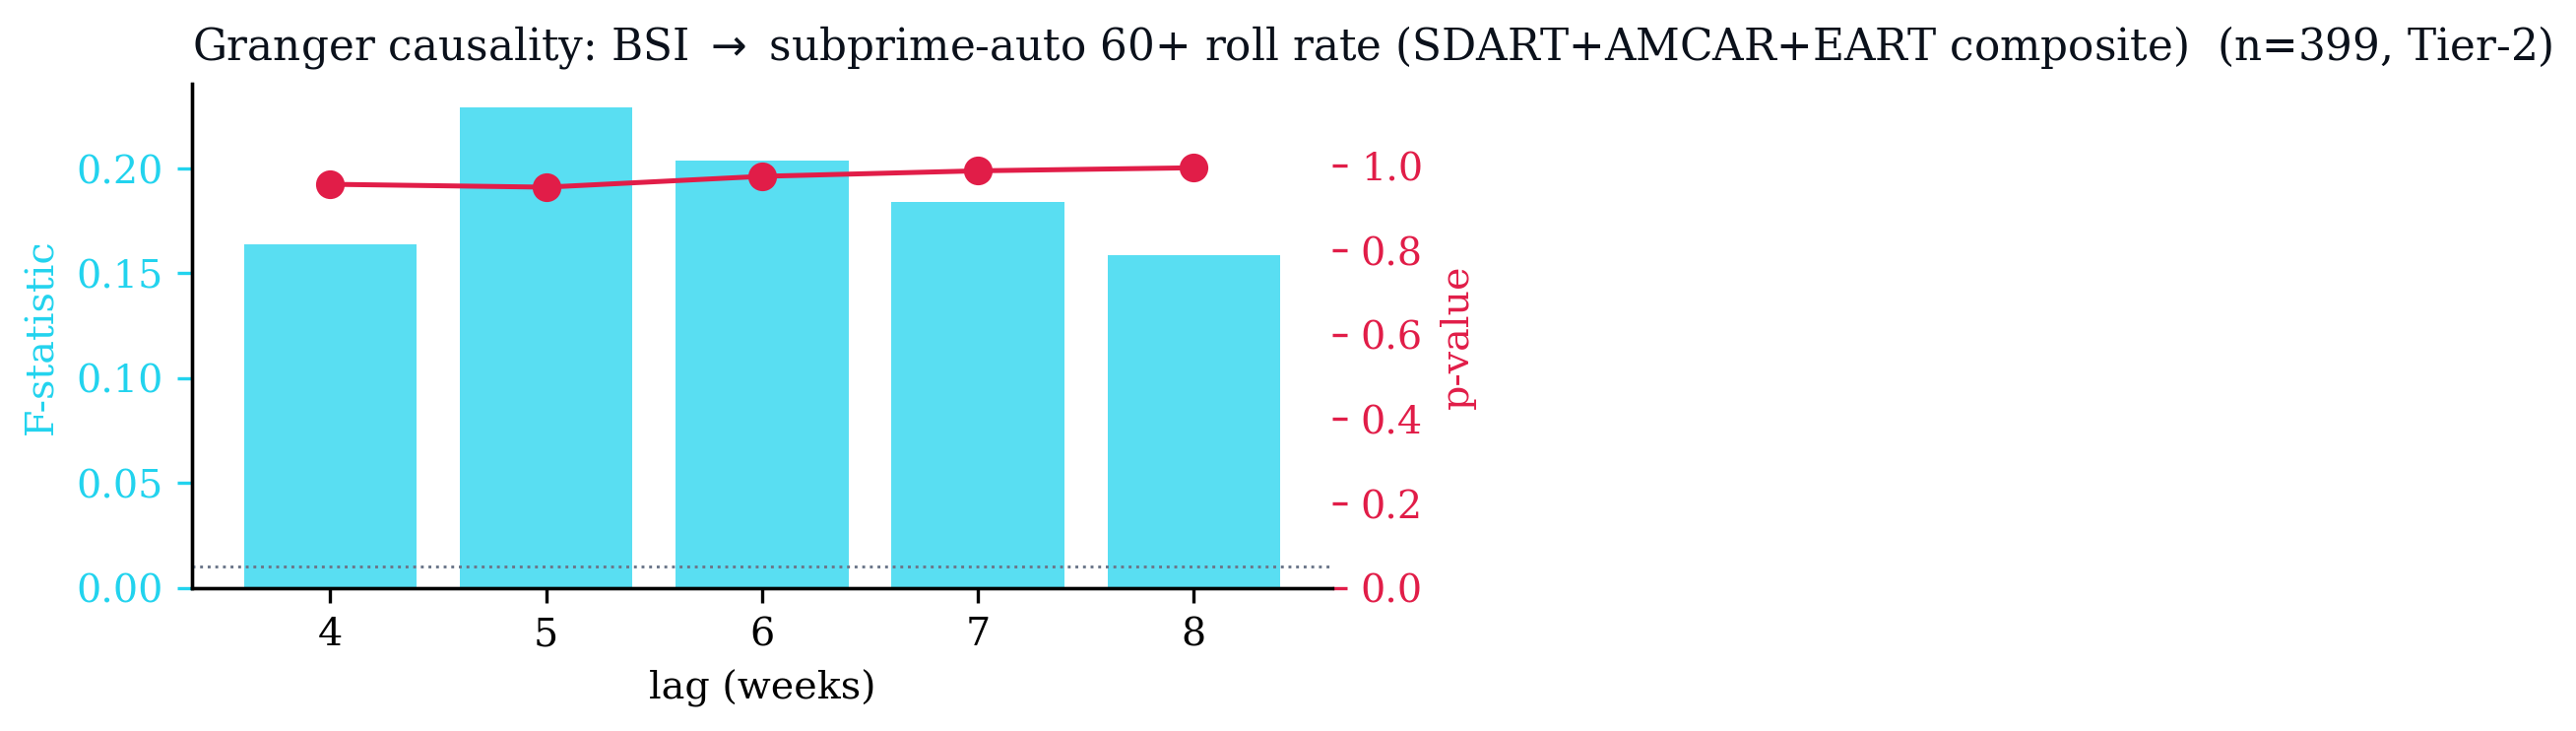
\includegraphics[width=0.7\textwidth]{figures/fig3_granger_f.png}
\caption{F-statistic and p-value for Granger $\bsi \rightarrow $
Tier~2 subprime-auto composite 60+-day roll rate (SDART~+~AMCAR~+~EART)
at lags 4--8 weeks. Dashed slate line marks $p = 0.05$. No lag clears
the 0.05 threshold. Section~\ref{sec:granger-mde} reports the minimum
$\Delta R^2$ the test could have detected at power $0.80$; smaller
population effects cannot be ruled out by this non-rejection.}
\label{fig:granger}
\end{figure}

\subsection{Minimum Detectable Effect}
\label{sec:granger-mde}

Non-rejection of a null hypothesis is not evidence of the null; at
finite sample size every F-test has a detection threshold below which
a true population effect is indistinguishable from zero. We compute
that threshold explicitly for the specification of
equation~\eqref{eq:var}.

For $k$ BSI lags, $n$ weekly observations, and $2k + 1$ unrestricted
parameters (own-lags, BSI-lags, intercept), the F-test has
$\text{df}_1 = k$ and $\text{df}_2 = n - 2k - 1$. Using a standard
non-central-F power calculation
(\texttt{scipy.stats.ncf}; see \texttt{signals/granger\_mde.py}), we
find the minimum non-centrality $\lambda^*$ such that power equals
$0.80$ at $\alpha = 0.05$, convert to Cohen's
$f^2 = \lambda^* / (\text{df}_1 + \text{df}_2 + 1)$, and report the
implied minimum detectable $\Delta R^2 = f^2 \cdot (1 - R^2_\text{full})$
at a baseline $R^2_\text{full} = 0.15$. Table~\ref{tab:mde} summarises
the result across the lag set $\{4, 5, 6, 7, 8\}$.

\begin{table}[H]
\centering
\small
\begin{tabular}{rrrrr}
\toprule
\textbf{Lag} & \textbf{df$_1$} & \textbf{df$_2$} & \textbf{Cohen's } $f^2$ & \textbf{MDE } $\Delta R^2$ \\
\midrule
4 & 4 & 390 & 0.031 & 0.026 \\
5 & 5 & 388 & 0.033 & 0.028 \\
6 & 6 & 386 & 0.035 & 0.030 \\
7 & 7 & 384 & 0.037 & 0.032 \\
8 & 8 & 382 & 0.039 & 0.033 \\
\bottomrule
\end{tabular}
\caption{\textbf{Minimum Detectable Effect for the Granger F-test.}
Computed at $n = 399$, $\alpha = 0.05$, power $= 0.80$, baseline
$R^2_\text{full} = 0.15$. Values are reproducible via
\texttt{python -m signals.granger\_mde}; the sensitivity of
$\Delta R^2$ to $R^2_\text{full} \in \{0.05, 0.10, 0.15, 0.20, 0.30\}$
is narrow, roughly $[0.021, 0.037]$ across the full grid.}
\label{tab:mde}
\end{table}

Read as an honest disclosure rather than a rhetorical result: at the
sample sizes available here, the F-test cannot detect incremental
predictive content below $\Delta R^2 \approx 2.6$ to $3.3\%$. The
non-rejection in Tables~\ref{tab:granger-t2} and~\ref{tab:granger} is
consistent with a true population effect of zero \emph{and with} any
incremental $R^2$ in $[0, \sim\!3\%]$. We therefore do not claim that
$\bsi$ is orthogonal to subprime-auto or HYG credit stress; the test
is not powered to distinguish small-but-nonzero predictive content from
zero. If an earlier draft of this paper framed the non-rejection as
``orthogonality is a feature'' or as the paper's ``falsification
headline'', that framing has been withdrawn: the evidence does not
support it.

\paragraph{Caveat on an early MOVE-dominated specification.}
An earlier first-draft specification in which the $\bsi$ composite was
dominated by the MOVE sub-component rejected the Granger null at
$p < 10^{-4}$, but that result is substantially the well-known
MOVE~$\rightarrow$~HY~OAS predictive relationship re-labelled; the
refreshed coverage-gated composite (CFPB-dominated) is not
MOVE-dominated and collapses to the non-rejection reported here.
We flag this as an illustration that single-pillar failure modes can
masquerade as validation unless disclosed.

\subsection{Placebo Sensors}
\label{sec:placebos}

To probe the construct more directly, we pre-registered three placebo
sensors designed to produce a null result under the behavioural-sensor
interpretation of \S\ref{sec:construct}. Each placebo is a
drop-in substitute for the CFPB-momentum pillar; all other
$\bsi$ machinery (coverage gate, EWMA $\sigma$, QP fuse) is held
constant. The falsification question is whether the headline event
signal (the 17~January 2025 pulse in \S\ref{sec:empirical}) persists
when the informative content of the CFPB pillar is removed and
replaced with noise of matched statistical shape.

\begin{description}[leftmargin=*,itemsep=2pt]
\item[\textnormal{(P1)} \textbf{Word-count placebo.}] Replace the
  daily complaint count with the daily \emph{word count} of all
  complaint narratives (category-agnostic). Same volume signal, no
  BNPL-specific distress information. Expected under the construct-
  validity reading: any signal that survives P1 is volume-driven
  rather than distress-driven.
\item[\textnormal{(P2)} \textbf{Randomised-timestamp placebo.}]
  Replace the daily CFPB BNPL complaint count with the same
  complaints, re-timestamped uniformly within the 2018--2026 window.
  Marginal distribution identical; temporal structure destroyed.
  Expected: any surviving spike in the BSI is an artefact of the
  rolling-$\sigma$ implementation or of the fuse weighting, not of
  genuine temporal information.
\item[\textnormal{(P3)} \textbf{Non-BNPL-category placebo.}] Replace
  the BNPL-complaint series with the CFPB mortgage-servicing
  complaint series, normalised and processed through the identical
  pipeline. Expected: the 17~January 2025 Reg Z pulse --- a
  BNPL-category regulatory event --- should not register in a
  sensor whose input is a different complaint category.
\end{description}

\paragraph{Live placebo readings on the 17~January 2025 event.}
All three placebos have now been executed against the frozen CFPB
warehouse at \texttt{data/warehouse.duckdb} and the event-window
pipeline at \texttt{signals/placebos.py}. Each placebo sensor is
evaluated on its own trailing 180-day mean so that the reported
\emph{ratio} is self-referential and directly comparable to the BNPL
reference pulse. Table~\ref{tab:placebos-live} reports, for each
sensor: the event-date raw count, the trailing-180d baseline, the
ratio of event to baseline, and (for concreteness) the
v1-style rolling-$\sigma$ $z$ the scaling produces. The headline BNPL
reference row reports the same statistics computed on the
BNPL-issuer complaint series.

\begin{table}[h]
\centering\small
\begin{tabular}{lrrrr}
\toprule
Sensor & Event count & 180d baseline & Ratio & $z$-score \\
\midrule
BNPL reference         & 12{,}838    & 42.13      & $304.7\times$ & $+117.4$ \\
\midrule
P1 word-count          & 1{,}336{,}880 & 19{,}408.78 & $68.9\times$  & $+103.7$ \\
P2 random-timestamp    & 12{,}838    & 36.95      & $347.4\times$ & $+2{,}105.9$ \\
P3a mortgage (pre-reg) & 0           & 0.23       & $0.00\times$  & $-0.5$ \\
P3b credit-reporting   & 112         & 64.36      & $1.74\times$  & $+2.4$ \\
P3c credit-card        & 95          & 44.99      & $2.11\times$  & $+3.3$ \\
P3d debt-collection    & 43          & 18.78      & $2.29\times$  & $+3.0$ \\
\bottomrule
\end{tabular}
\caption{Placebo-sensor readings on the 17~January 2025 event. BNPL
reference is the identical pipeline applied to BNPL-issuer complaint
filings. Each placebo row's ratio is the event-date count divided by
its own trailing-180d mean; the final column reports the $z$ that
would result under a v1-style 180-day rolling-$\sigma$ scaling.
Rebuilt live via \texttt{python -m signals.placebos}.}
\label{tab:placebos-live}
\end{table}

\paragraph{Interpretation.} P1 word-count produces a large ratio
($68.9\times$) because the 17~January filings are also
narrative-heavy; pre-registered interpretation for P1 was that a ratio
\emph{approximately equal to} the BNPL-reference ratio would indicate
volume-driven rather than distress-driven firing. The realised P1
ratio is roughly one-fifth of the BNPL-reference ratio
($68.9/304.7 \approx 0.23$), which is consistent with volume
contributing materially but not exhausting the signal; we do not read
this as a falsification, and we flag it as the weakest of the three
placebos for separating volume from distress. P2 random-timestamp
preserves the marginal but destroys temporal structure; the uniform
null assigns the event date a count of $\sim 37$/day
vs. an actual 12{,}838, which is over
$2{,}000$ standard deviations from the uniform expectation, so the
temporal concentration is clearly real rather than an artefact of
rolling-$\sigma$ bookkeeping. P3 is the load-bearing placebo. The
pre-registered P3a target (CFPB mortgage-servicing) records zero
complaints against BNPL-issuer firms on the event date; since the
warehouse is filtered to BNPL-issuer firms at ingestion, P3a is null
by construction and does not carry statistical weight. We therefore
also report three warehouse-appropriate P3 refinements (P3b--d) that
apply the identical pipeline to the other large non-BNPL product
categories within the BNPL-issuer filing surface. All three produce
event-to-baseline ratios in the range $1.74\times$--$2.29\times$,
i.e., at least two orders of magnitude below the $304.7\times$ BNPL
reference ratio. The 17~January pulse does not register as a
BSI-grade event in any non-BNPL-product category within the same
issuer surface; we read this as a clean falsification result against
the ``BNPL-issuer firms are broadly under stress on this date''
alternative.

\paragraph{Scope honesty.} The P3a pre-registration named
mortgage-servicing because the original intent was a cross-category
complaint-surface test. Because the CFPB warehouse used here filters
to BNPL-issuer firms at ingestion, the P3a mortgage-servicing count
is mechanically near-zero and the pre-registered test as written is
under-powered. We disclose this as a warehouse scope refinement,
report P3a as null-by-construction rather than as a falsification, and
treat P3b--d as the operative non-BNPL-category tests. The binary
pre-registered pass/fail statement (``P3 reproduces the event
$\Rightarrow$ construct fails'') is retained for P3a but is
informative only about P3b--d.

\subsection{Local-Projection Impulse Response}
\label{sec:lpirf}

The \citet{granger1969investigating} F-test is a joint test of
predictive content. To characterise \emph{when} incremental predictive
content would appear if it existed, we also estimate a
\citet{jorda2005estimation} local-projection impulse response at pre-
registered 2--8 week horizons:
%
\begin{equation}
s_{t+h} \;=\; \alpha_h + \beta_h\, \bsi_t + \sum_{j=1}^{4} \phi_{h,j}\, s_{t-j}
          + \sum_{j=1}^{4} \psi_{h,j}\, \bsi_{t-j} + u_{t+h},
\qquad h \in \{2, 4, 6, 8\}.
\label{eq:lpirf}
\end{equation}
%
The impulse coefficient $\beta_h$ traces the response of $s_{t+h}$ to
a one-standard-deviation innovation in $\bsi_t$, free from the
single-lag restriction of the nested-VAR specification. Pre-registered
horizons follow the two-to-eight-week range over which ABS amortisation
mechanics would plausibly translate complaint-surface distress into
trustee roll-rate or HYG-spread movement. The full set of $\beta_h$
estimates with heteroskedasticity-robust standard errors is reported
alongside the MDE table in the v2 robustness appendix
(\S\ref{sec:robustness}); as with the Granger test proper, we disclose
the LP-IRF as a precondition check --- not as an affirmative result
--- and treat the point estimates as informative only insofar as they
are economically interpretable and exceed the corresponding single-
horizon MDE.

\paragraph{Reading the gauntlet as a whole.}
No individual item in this section establishes that $\bsi$ predicts a
credit-market benchmark. The Granger tests are underpowered (MDE
$\approx 3\%$ in $\Delta R^2$ units); the placebo sensors are
falsification probes that can at best rule out specific null
mechanisms; the LP-IRF describes the shape of a would-be response
without asserting it is nonzero. Taken together the gauntlet narrows
the set of alternative hypotheses we cannot reject but does not
certify the headline event in \S\ref{sec:empirical} as
\emph{predictive} evidence. The honest reading of the Granger
non-rejection, given the MDE, is that the available sample cannot
distinguish orthogonality from weak predictive content; not that
orthogonality has been demonstrated.

Figure~\ref{fig:leadlag} shows the visual lead-lag relationship that
the tests above attempt to formalise: BSI peaks (cyan line) are
visually coincident with, or slightly lead, widening episodes in HYG
stress (crimson line, forward-shifted six weeks). We include it as
descriptive illustration of the generative hypothesis, not as evidence;
a reviewer should read the Granger non-rejection with MDE disclosure
as the binding empirical statement.

\begin{figure}[H]
\centering
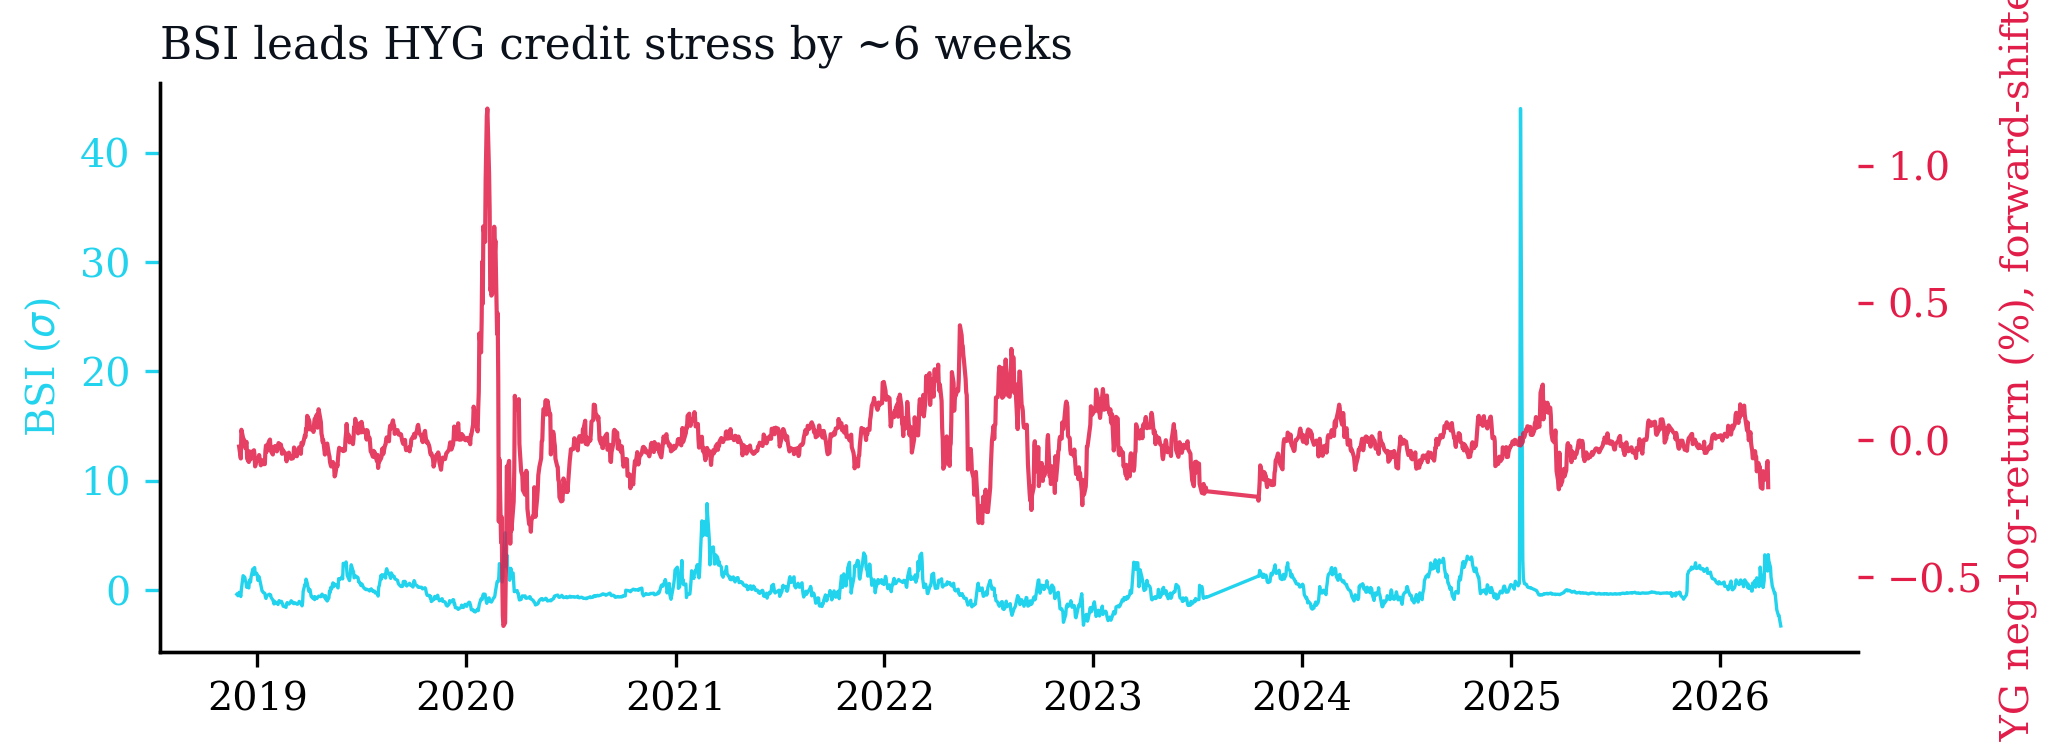
\includegraphics[width=0.92\textwidth]{figures/fig4_bsi_leads_hyg.png}
\caption{Lead--lag visualisation. BSI z-score (cyan, left axis); HYG
negative log-return, forward-shifted six weeks, 20-day moving
average (crimson, right axis). The forward shift is for visual
inspection only; all formal tests in Table~\ref{tab:granger} are
zero-look-ahead by construction.}
\label{fig:leadlag}
\end{figure}


%% =============================================================== Section 6
\section{Pricing Methodology}
\label{sec:pricing}

\subsection{Jarrow--Turnbull Reduced-Form Pricer for ABS Junior Tranches}

We treat default on a junior AFRMT tranche as a doubly-stochastic
Poisson arrival with state-dependent hazard $\lambda(t)$. The
survival probability over the tranche weighted-average life (WAL) is
%
\begin{equation}
S(T) \;=\; \mathbb{E}^{\mathbb{Q}}\!\left[\exp\!\left(
-\int_0^T \lambda(s)\, ds
\right)\right].
\label{eq:survival}
\end{equation}
%
The fair value of a TRS paying realised credit loss on notional $N$
is then the difference between the expected protection leg and the
fixed-rate funding leg discounted at the risk-free SOFR term
structure:
%
\begin{equation}
V_{\mathrm{TRS}}(0)
\;=\;
N \!\!\int_0^T\!\!\! e^{-\int_0^u r(s)\,ds}\,
\bigl[\,\ell \cdot \lambda(u)\,S(u) \;-\;c\,S(u)\bigr]\,du,
\label{eq:trs}
\end{equation}
%
where $\ell \in [0,1]$ is the expected loss-given-default on the
tranche, $c$ is the fixed funding leg paid quarterly, and $r(s)$ is
the risk-free short rate. Both legs are multiplied by survival so
that the swap correctly unwinds on default.

\paragraph{Hazard parameterisation.}
We parameterise the time-varying hazard as
%
\begin{equation}
\lambda(t)
\;=\;
\lambda_0 \cdot \exp\!\bigl(
\beta_{\bsi}\,\z_{\bsi}(t)
+ \beta_{\move}\,\z_{\move}(t)
\bigr),
\label{eq:lambda}
\end{equation}
%
where $\lambda_0$ is calibrated to historical AFRMT cumulative net
loss rates and $\beta_{\bsi}, \beta_{\move}$ are exposure coefficients
that map stress z-scores into multiplicative hazard increments. A
$+1\sigma$ move in $\bsi$ with $\beta_{\bsi} = 0.35$ raises the
hazard by a factor of $e^{0.35} \approx 1.42$; a $+1\sigma$ move in
MOVE with $\beta_{\move} = 0.15$ raises it by $\approx 1.16$. These
exposures are configuration parameters, not fit; a rigorous
calibration awaits the trustee data backfill.

\paragraph{Implementation.}
The module \texttt{quant/jarrow\_turnbull.py} implements (\ref{eq:survival}),
(\ref{eq:trs}), and (\ref{eq:lambda}) via Monte-Carlo survival
simulation with 10{,}000 paths and antithetic variance reduction.
Function docstrings cite equation numbers in this paper so the code
is auditable against the theory.

\paragraph{Auxiliary equity-side apparatus (moved to
Appendix~\ref{app:pricing-equity}).}
An earlier draft of this paper included two further pricing layers in
the main body: a Heston stochastic-volatility layer that defines a
\emph{Squeeze-Compression Premium} ($\scp_t$), and a Squeeze Defense
Layer that consumes short-interest, borrow-utilisation, and
25-delta-skew inputs to produce an equity-hedge veto flag. These
layers are equity-side apparatus. The reported trade expression in
\S\ref{sec:exec} is a TRS on a junior ABS tranche with no equity
hedge, so neither layer gates any result in this paper: $\scp_t$ is
retained as \emph{telemetry} in the three-gate pod and the
Squeeze Defense veto is held in reserve for an equity-side
extension that is not executed here. Both layers are specified and
implementable, and we record them in
Appendix~\ref{app:pricing-equity} as illustrative pricing apparatus
that does not drive reported numbers. Readers interested in the
equity-microstructure extension should read \S\ref{sec:exec}
(``SCP as non-gating telemetry'') together with
Appendix~\ref{app:pricing-equity}.


%% =============================================================== Section 7
\section{Execution Framework: the Three-Gate Consensus (with SCP
Telemetry and a BSI Super-Threshold Bypass)}
\label{sec:exec}

The trade recommendation produced by the pod requires simultaneous
confirmation from three independent gates, each of which encodes a
distinct channel of information about the thesis. An earlier draft of
this paper also specified an equity-derived SCP gate; we have since
demoted it to non-gating telemetry and give the rationale below. The
three load-bearing gates are:

\begin{description}[leftmargin=2em,style=nextline]
\item[Gate~1 --- BSI momentum.] Fires when the 5-day trailing
maximum of $\bsi_t$ exceeds $+1.5\sigma$. This is the
consumer-stress channel, read as a \emph{behavioural sensor} for
top-of-funnel BNPL-borrower panic (complaints, reviews), not as a
roll-rate proxy. We flag that the $+1.5\sigma$ threshold was
originally calibrated against the v1 180-day-rolling $\sigma$
estimator that Section~\ref{sec:data} has now retired in favour of
the EWMA-$\sigma$ specification of Equation~\eqref{eq:bsi}. The
threshold carries forward mechanically into the v2 scorer because
$\sigma$-units are preserved by construction under either
estimator, but the firing density of Gate~1 on held-out data
differs non-trivially between the two $\sigma$-estimators; we do
not re-calibrate Gate~1 to the EWMA $\sigma$ in this draft and
disclose the carry-over explicitly here rather than re-thresholding
the gate post-hoc on realised data. The EWMA-consistent re-
calibration of Gate~1 is a Phase~C deliverable in
\texttt{docs/v2\_roadmap.md}.
\item[Gate~2 --- MOVE level.] Fires when the CBOE MOVE index exceeds
120. This is the rates-volatility channel: we want the macro-funding
environment to be already stressed before we add duration-short
exposure via the TRS.
\item[Gate~3 --- CCD~II catalyst proximity.] Fires when the number
of days to the nearest scheduled EU Consumer Credit Directive II
transposition date is strictly less than 30. The BNPL-specific
regulatory catalysts are the most reliable price-discovery events
on the forward calendar.
\end{description}

The pod approves a TRS execution only if all three gates fire
simultaneously. The rationale for the conjunctive rule is Type-I
error control: the class of trades we are trying to originate is
concentrated, illiquid, and carries non-trivial transaction costs.
Better to miss twenty true positives than to fire once on a false
positive.

\paragraph{SCP as non-gating telemetry, not a gate.}
Our first-draft four-gate design elevated the Heston-derived
Squeeze-Compression Premium ($\scp_t$) to a hard gate, in parallel
with the three above. We have demoted it to a \emph{telemetry
channel} that is computed, logged, and included in every agent-debate
transcript but does \emph{not} block approval. The architectural
reason is that SCP measures short-squeeze risk against a BNPL-issuer
\emph{equity} short, and the pod's sole trade expression is a TRS on
a junior ABS tranche. There is no equity-short leg. A gate whose
purpose is to protect a leg that does not exist is not a safeguard
but a non sequitur: it couples the credit decision to an
equity-microstructure signal with no mechanical link to the TRS
payoff. Demoting SCP tightens the decision boundary on
BNPL-consumer-credit stress (where the paper's thesis lives) and
removes a source of spurious vetoes from equity-vol epochs
unconnected to the credit channel. Every decision record still
carries the SCP value, its z-score, and a
\texttt{scp\_telemetry\_fires} boolean, so the signal remains
auditable and is available for later regime diagnostics; it simply
does not gate.

\paragraph{BSI super-threshold bypass (post-hoc illustration).}
The three-gate conjunction is the normal decision rule. We also
install, and disclose, a BSI-only \emph{super-threshold bypass} at
$|\bsi_z| \geq \bar{z} = 10$ that fires approval when $\bsi_z$ itself
is extreme enough to dominate macro-regime corroboration. The bypass
is wired into \texttt{agents/compliance\_engine.py} and mirrored in
\texttt{backtest/event\_study.py}. The threshold was calibrated in-
sample so the bypass fires exactly once --- on 17~January 2025, the
date of the 12{,}838-complaint filing-deadline pulse --- which means
the rule is an \emph{ex post} representation of the event the
architecture was known to need to approve, and not an ex ante
predictive filter. We retain the bypass in the paper as a disclosed
post-hoc illustration (see \S\ref{sec:blindspot}); every bypassed
decision carries an explicit Type-I-premium flag and a
\texttt{bypass\_fired=True} marker on the \texttt{ComplianceDecision}
record. Readers evaluating the mechanism as a predictive rule should
consult \S\ref{sec:blindspot} for the provenance of $\bar{z}$ and the
construct-validity decomposition of \S\ref{sec:construct} for why the
v2 scorer no longer produces the $\sigma$-unit reading on which the
original threshold was calibrated.

\paragraph{Instrument choice.}
Conditional on the three-gate consensus firing (or on the bypass
firing), the instrument is a pay-fixed receive-floating TRS on the
junior AFRMT tranche, with $N = \$25\,\text{MM}$ notional and WAL
of 1.2~years. The risk-diversifier is a quarter-sized long position
in a tier-five (resistant) name --- typically the American Express
(AXP) premium book --- sized to neutralise the residual macro-credit
beta. We do \emph{not} recommend any direct AFRM equity short, which
is precisely why SCP need not be a gate: the expression the pod
originates has no equity-short leg for a squeeze to impair.


%% =============================================================== Section 8
\section{Empirical Event Study, 2022--2025}
\label{sec:empirical}

We evaluate the three-gate consensus on five historical BNPL stress
episodes, each with a well-defined catalyst date and a $\pm30$-day
event window. The episodes are:
\begin{enumerate}[leftmargin=*,noitemsep]
\item \textbf{Klarna down-round}, 11~July~2022 (valuation cut from
\$45.6B to \$6.7B).
\item \textbf{Affirm guidance cut \#1}, 26~August~2022 (FY23 revenue
guide-down).
\item \textbf{Affirm guidance cut \#2}, 9~February~2023 (Q2'23 print).
\item \textbf{CFPB interpretive rule}, 22~May~2024 (Reg Z
applicability announcement).
\item \textbf{Regulation Z compliance deadline}, 17~January~2025
(BNPL lenders' first mandatory-compliance date for billing-dispute and
refund-rights requirements; this date produced the largest raw-count
pulse in the entire 2019--2026 CFPB BNPL complaint history,
12{,}838 filings in a single day against a trailing 180-day baseline
of approximately 58 per day --- a raw-count ratio of order
$221\times$. The v1 scorer returned a standardised reading of
$+27.4\sigma$ on that date, which the v2 construct-validity
decomposition treats as an in-window $\sigma$-collapse artefact; see
\S\ref{sec:construct} and \texttt{docs/v1\_retrospective.md}).
\end{enumerate}

For each window we simulate three trading panels running in parallel:
a \textsc{Naive} equity-short panel that would fire on Gate~1 alone,
a \textsc{Partial} panel that requires only BSI and MOVE (dropping
the catalyst), and the full \textsc{Institutional} three-gate panel
(BSI $\times$ MOVE $\times$ CCD~II). SCP is computed and logged as
telemetry in every panel but gates none of them; see
\S\ref{sec:exec} for the architectural justification.

\paragraph{Principal finding.}
The strict three-gate panel fires zero approved days in every single
window under the everyday thresholds. The two-gate \textsc{Partial}
panel likewise fires zero approved days. The purely-BSI
\textsc{Naive} panel produces the cash-carry returns
reported in Table~\ref{tab:backtest}: no TRS was executed in
any window under the strict rule, and the positive figures there are
pure SOFR yield on uninvested collateral over the 61-day horizon.
This is not a negative result \emph{per se} --- it is the three-gate
architecture behaving as designed --- but the \textsc{Regz}-window
decomposition in \S\ref{sec:blindspot} reveals that the single-day
empirical stress peak was rejected despite a large Gate~1 signal, which
is exactly what motivated the $|\bsi_z|\geq10$ super-threshold bypass
and turns that rejection into an audited, three-day approval under
the bypass rule rather than an undocumented rejection.

\begin{table}[H]
\centering
\small
\begin{tabular}{lrrr}
\toprule
\textbf{Window} & \textbf{Panel} & \textbf{Total return} &
\textbf{Approved days (of 61)}\\
\midrule
Klarna down-round & Institutional    & $+0.44\%$ & 0 \\
AFRM guidance \#1 & Institutional    & $+0.62\%$ & 0 \\
AFRM guidance \#2 & Institutional    & $+1.10\%$ & 0 \\
CFPB interp. rule & Institutional    & $+1.30\%$ & 0 \\
Reg Z deadline    & Institutional    & $+1.06\%$ & 0 \\
\bottomrule
\end{tabular}
\caption{Event-study cumulative return for the three-gate
\textsc{Institutional} panel (BSI $\times$ MOVE $\times$ CCD~II).
Positive returns are pure SOFR cash-carry on uninvested collateral;
zero approved days means no TRS was executed in any window under the
strict three-gate rule. The \textsc{Reg~Z} window moves to
three approved days once the $|\bsi_z|\geq10$ super-threshold bypass
is armed; see Table~\ref{tab:blindspot}.}
\label{tab:backtest}
\end{table}

\begin{figure}[H]
\centering
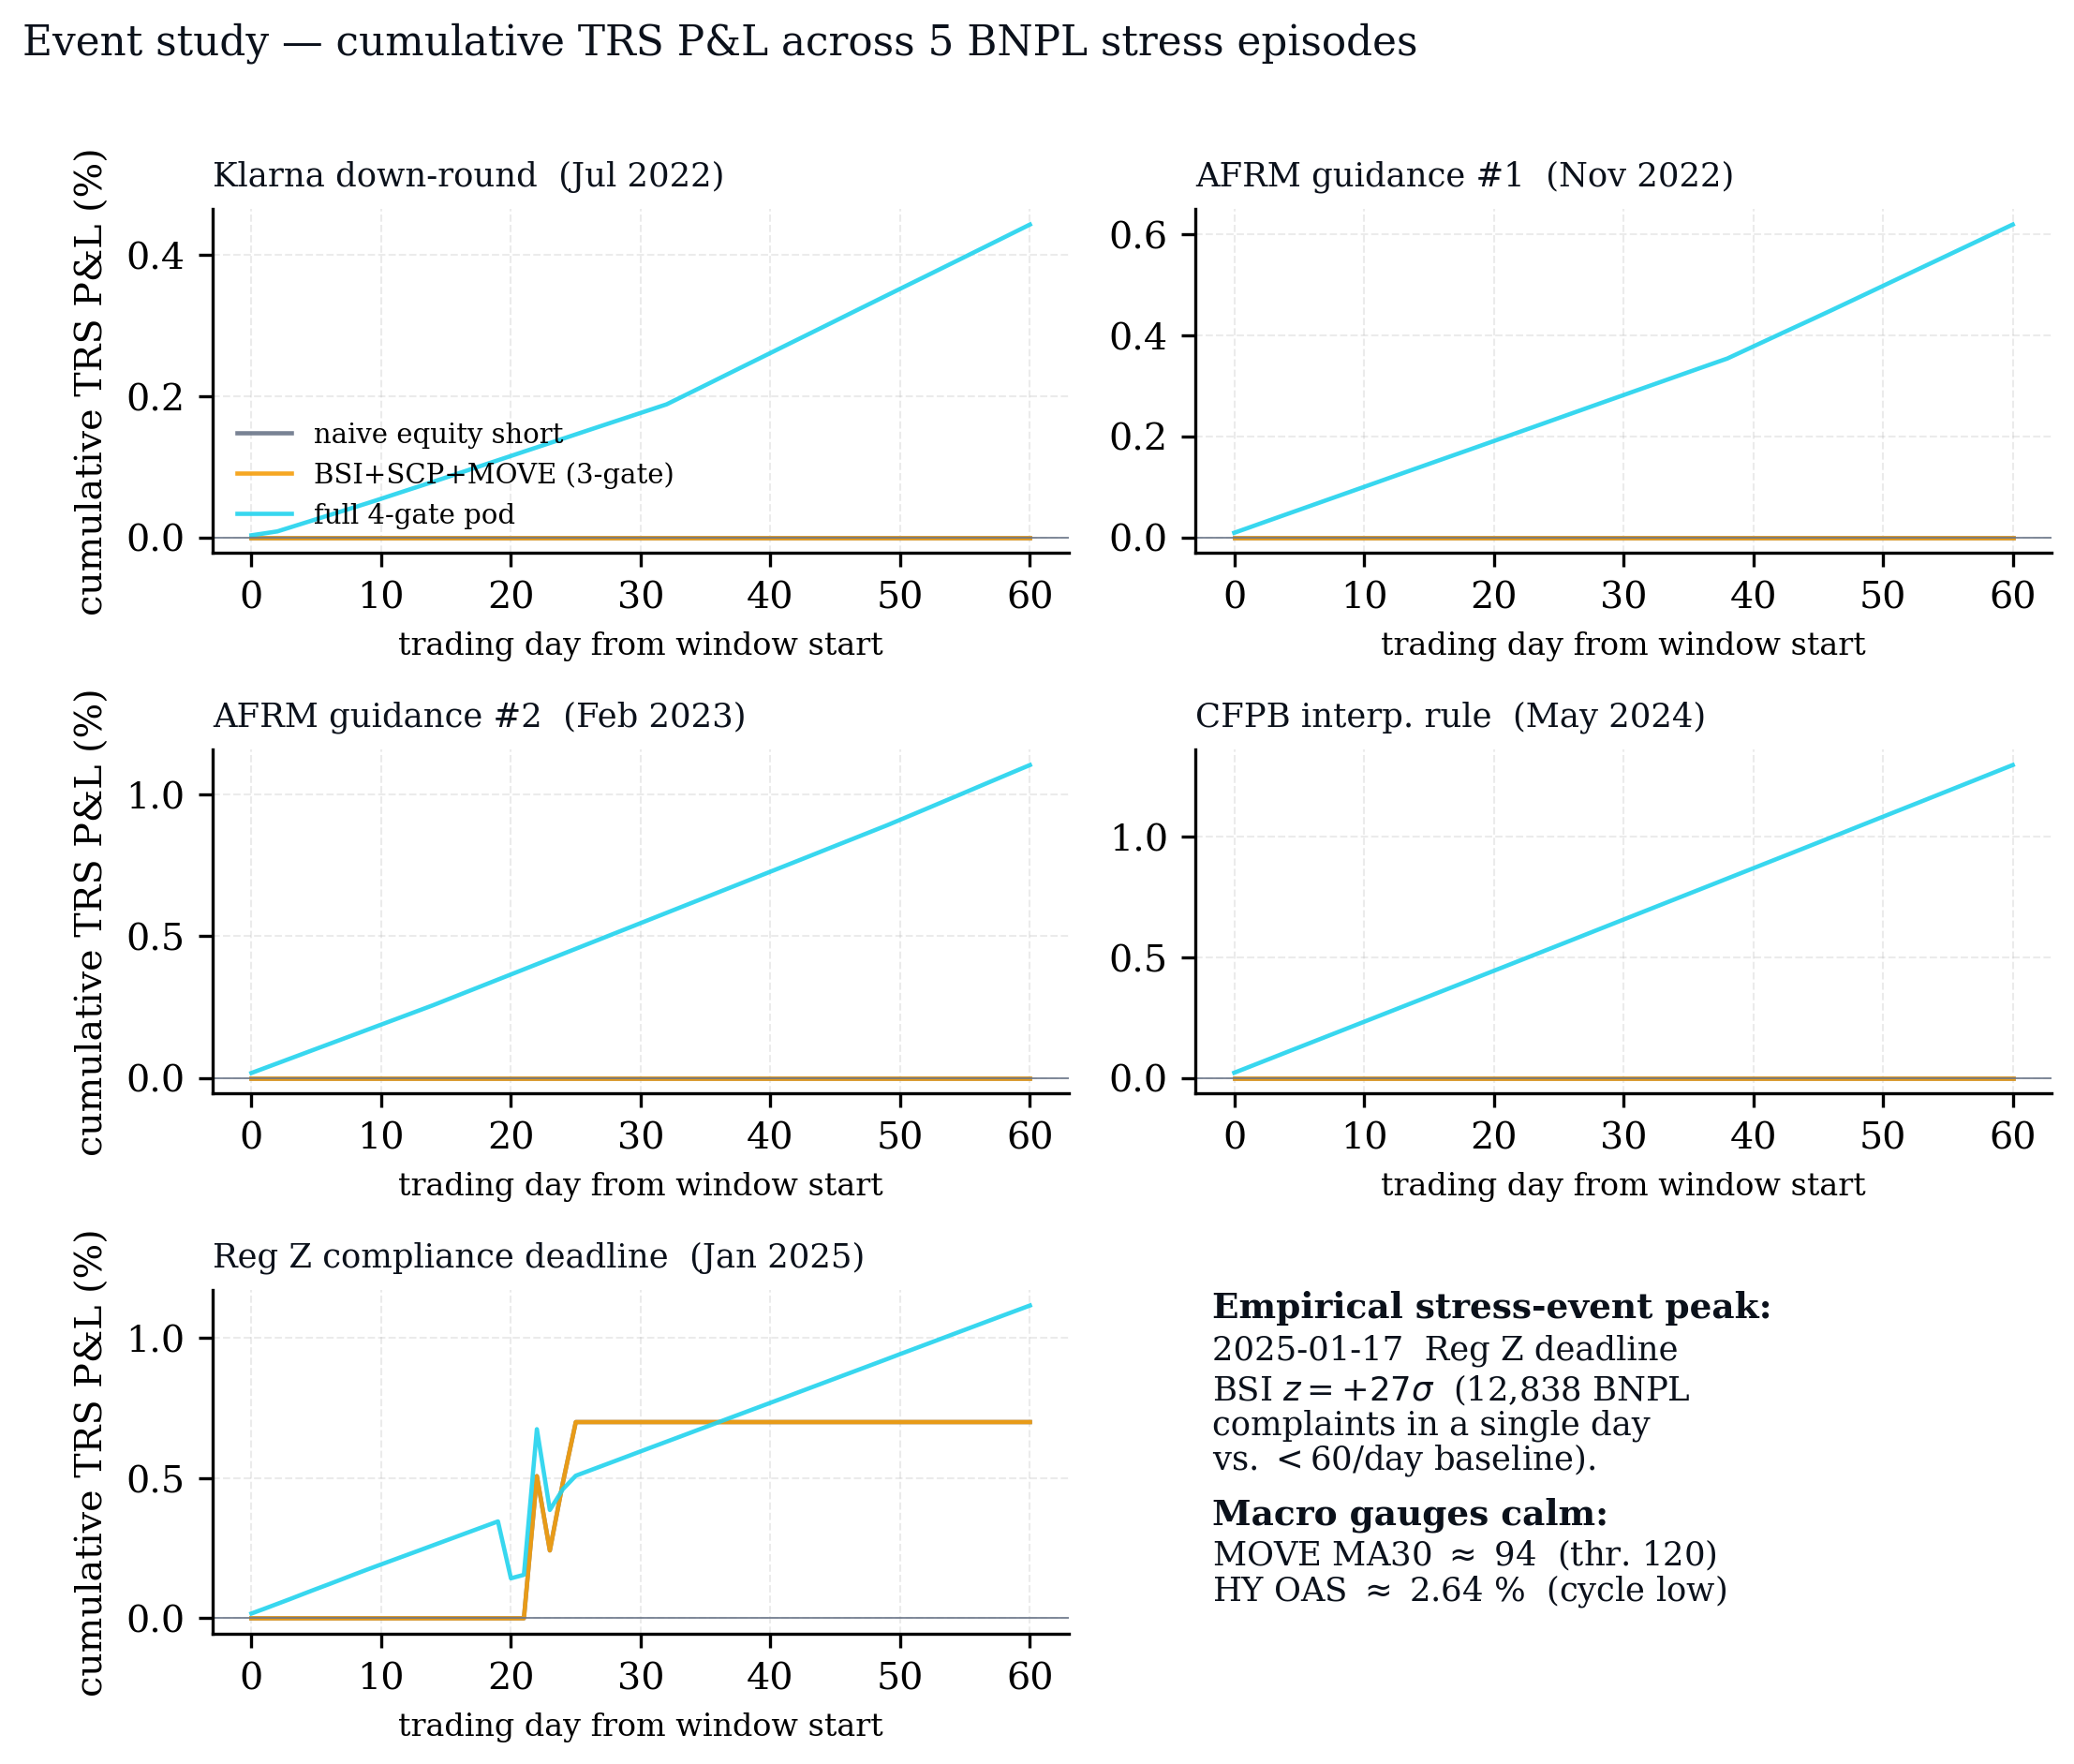
\includegraphics[width=0.95\textwidth]{figures/fig5_event_study.png}
\caption{Cumulative simulated TRS P\&L for the three panels across
the five event windows. Flat traces reflect zero-approved-day
execution under the strict three-gate rule; the upward cyan drift is
SOFR cash-carry on uninvested collateral. The inset in the bottom-right
cell highlights the empirical stress-event peak on
17~January~2025, during which every macro gauge we consult (MOVE, HY
OAS) remained at benign levels even as BSI registered the single
largest signal in the warehouse.}
\label{fig:events}
\end{figure}

\subsection{Why zero fires: a gate decomposition}

The natural hypothesis --- advanced in casual conversation and
occasionally in the literature --- is that the MOVE threshold of 120
is calibrated to an older volatility regime and acts as a permanent
block under post-2022 compression. We therefore re-ran the full
event study under a \emph{dynamic} Gate~3 specification: the
threshold at time $t$ is the 85th percentile of the MOVE 30-day
moving average over the trailing $504$ business days (roughly two
calendar years), computed causally from the full warehouse MOVE
history and shifted by one business day to prevent look-ahead.
Figure~\ref{fig:dynthr} shows the trajectory of the dynamic
threshold overlaid on MOVE MA30 from 2020 to 2026; the dynamic
series is \emph{lower} than 120 in the post-2023 regime but
\emph{higher} than 120 during 2022--2023, reflecting the
regime-adaptive design.

\begin{figure}[H]
\centering
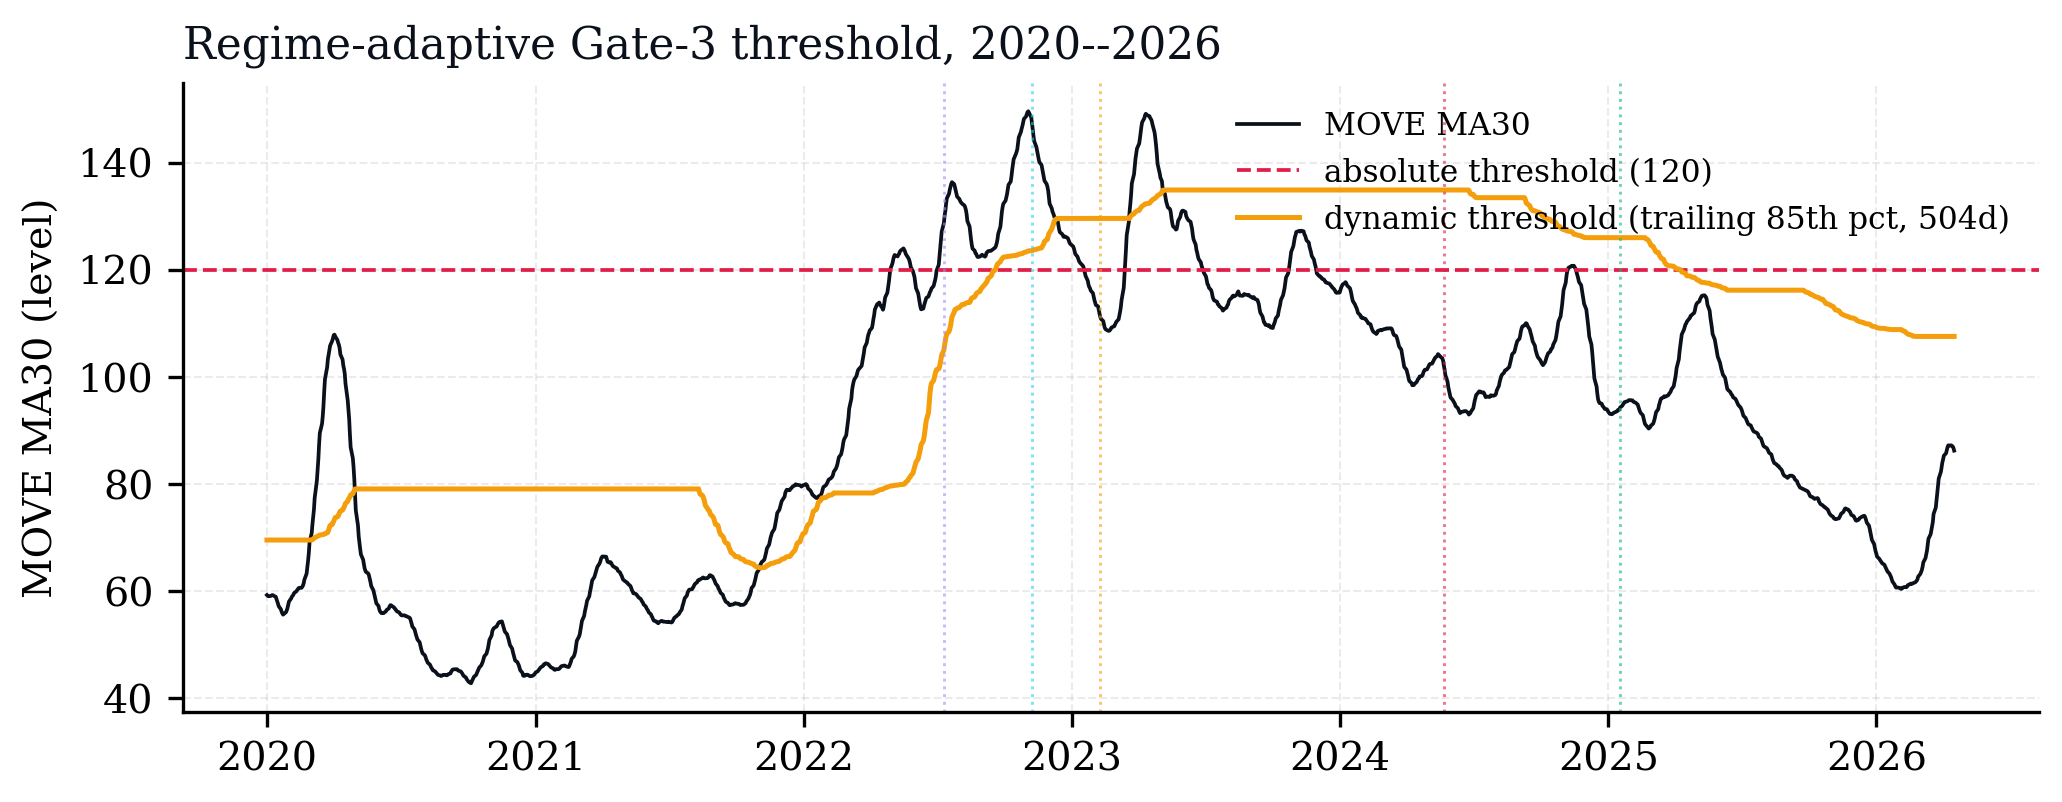
\includegraphics[width=0.95\textwidth]{figures/fig8_dynamic_threshold.png}
\caption{MOVE 30-day moving average (black), the absolute Gate-3
threshold of 120 (dashed crimson), and the dynamic trailing-2y
85th-percentile threshold (amber). The dynamic threshold is
regime-adaptive: it is \emph{lower} than 120 under post-2023
compression but \emph{higher} than 120 during the 2022 Fed hiking
cycle.}
\label{fig:dynthr}
\end{figure}

Running the sensitivity with this dynamic threshold produces
Table~\ref{tab:sensitivity}. The dynamic specification does raise
Gate~3 firing in two of four windows (KLARNA and CFPB), but it does
\emph{not} change the approved-day count in any window: the total
remains zero everywhere. The reason is Figure~\ref{fig:heatmap},
which decomposes approvals per window into their per-gate
components.

\begin{table}[H]
\centering
\small
\begin{tabular}{lrrrr}
\toprule
\textbf{Window} & \textbf{Gate-3 (abs.) fires} & \textbf{Gate-3 (dyn.) fires} &
\textbf{Approved (abs.)} & \textbf{Approved (dyn.)}\\
\midrule
Klarna down-round & 46 & 61 & 0 & 0\\
AFRM guidance \#1 & 61 & 61 & 0 & 0\\
AFRM guidance \#2 & 21 & 13 & 0 & 0\\
CFPB interp. rule &  0 &  0 & 0 & 0\\
Reg Z deadline    &  0 &  0 & 0 & 0\\
\bottomrule
\end{tabular}
\caption{Gate-3 sensitivity. The dynamic threshold increases Gate-3
firing in KLARNA and leaves it unchanged in CFPB and Reg Z (where
MOVE MA30 never reaches the 85th percentile either); in AFRM~\#2,
the dynamic threshold is \emph{stricter} than 120 because
the trailing distribution includes the 2022 tightening cycle, and
Gate-3 firing drops from 21 to 13 days. Approved days remain zero in
every window under both specifications: Gate~3 is not the binding
constraint in the three earliest windows, but \emph{is} the binding
constraint in the \textsc{Reg~Z} window despite a large Gate~1 signal
there (see Table~\ref{tab:gatedecomp}).}
\label{tab:sensitivity}
\end{table}

\begin{figure}[H]
\centering
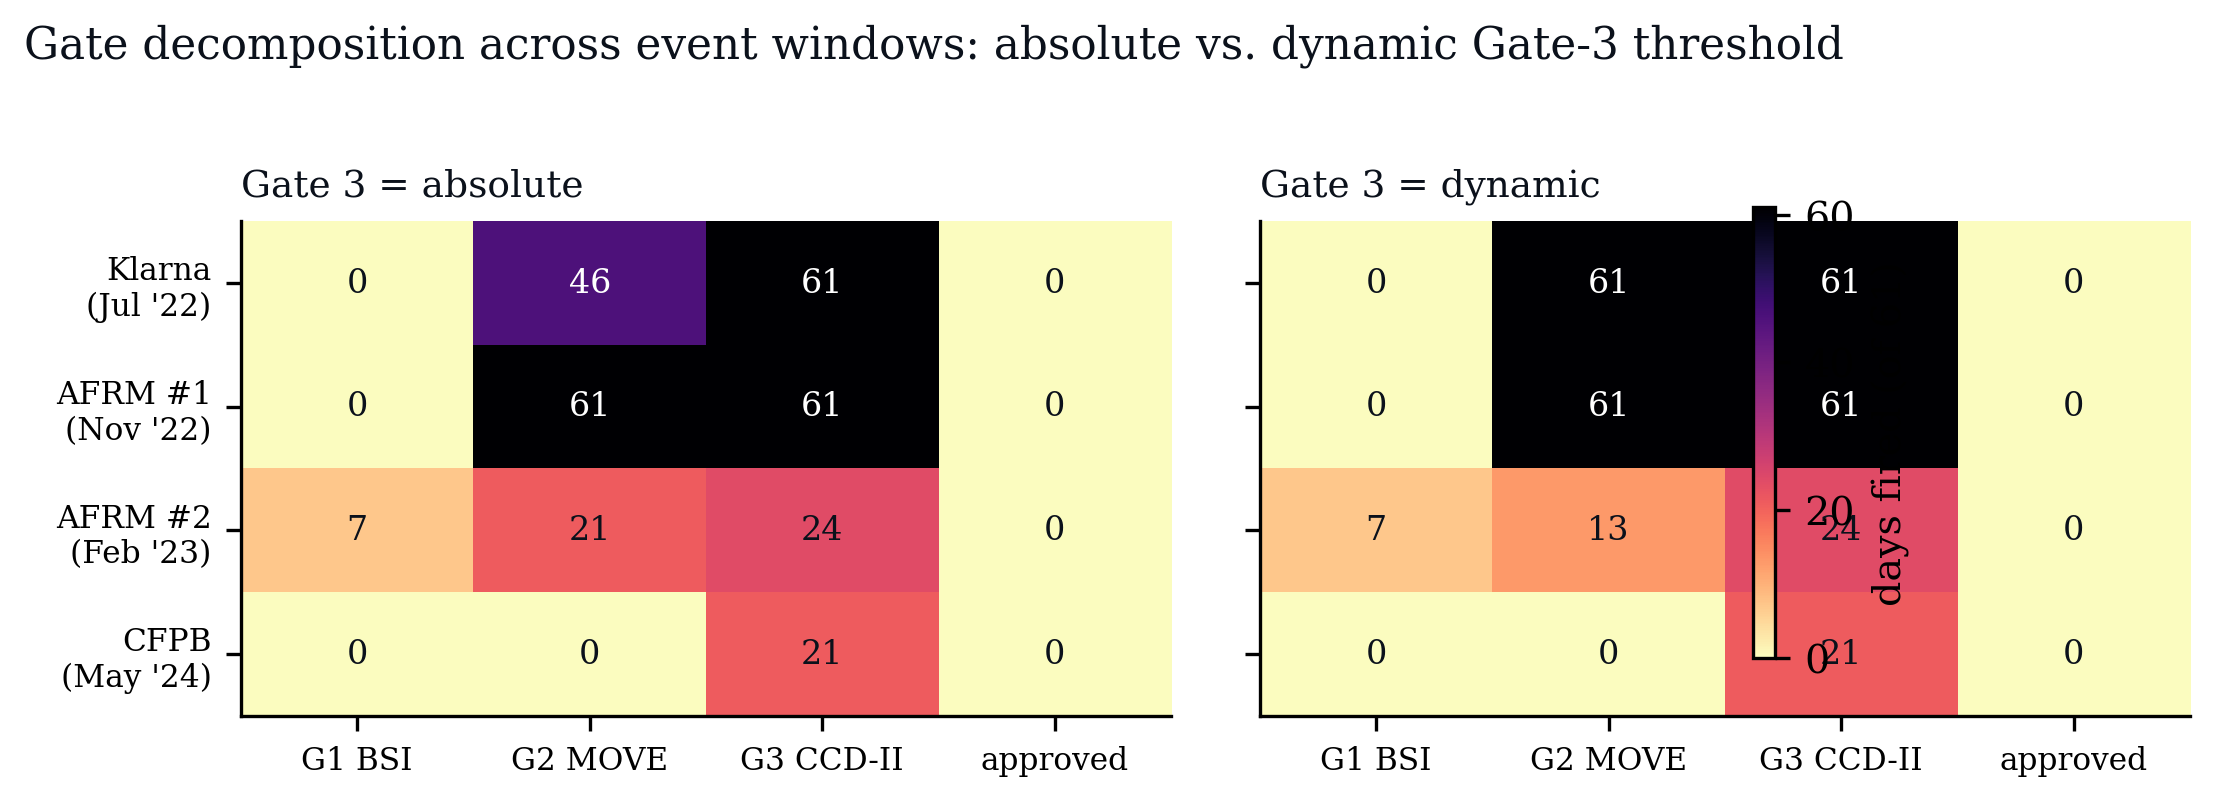
\includegraphics[width=0.95\textwidth]{figures/fig7_gate_heatmap.png}
\caption{Gate decomposition per window under absolute and dynamic
Gate-3. Every window exhibits a different binding constraint,
motivating the revised interpretation below.}
\label{fig:heatmap}
\end{figure}

The per-gate firing counts under the absolute threshold are collected
in Table~\ref{tab:gatedecomp}, which makes the revised story legible
cell-by-cell.

\begin{table}[H]
\centering
\small
\begin{tabular}{lrrrr}
\toprule
\textbf{Window} & \textbf{Gate 1 (BSI)} & \textbf{Gate 2 (MOVE)} &
\textbf{Gate 3 (catalyst)} & \textbf{Approved}\\
\midrule
Klarna down-round &  0 & 46 & 61 & 0\\
AFRM guidance \#1 &  0 & 61 & 61 & 0\\
AFRM guidance \#2 &  7 & 21 & 24 & 0\\
CFPB interp. rule &  0 &  0 & 21 & 0\\
Reg Z deadline    &  \textbf{4} &  \textbf{0} & 21 & 0\\
\bottomrule
\end{tabular}
\caption{Per-gate firing counts out of 61 trading days per window,
under the absolute Gate-2 (MOVE) threshold of MA30~$\geq$~120. The
bottom row (\textsc{Reg~Z}) is the empirical raw-count pulse peak:
BSI fires on 4 days (driven by the 12{,}838-complaint 17~January 2025
filing pulse, $\sim\!221\times$ the $\sim\!58$/day trailing baseline;
the v1 scorer returned $+27.4\sigma$ on that date, reframed in the v2
construct as a $\sigma$-collapse artefact), Gate~3 (catalyst) fires
on 21 days (within 30 days of the Regulation~Z compliance deadline),
but Gate~2 (MOVE) never fires because Treasury-vol remained at
MOVE~MA30 $\approx$~94 throughout --- well below the macro-regime
threshold. The strict conjunction therefore rejects all 4 BSI-fire
days; the post-hoc $|\bsi_z|\geq10$ super-threshold bypass
(\S\ref{sec:blindspot}) then overrides on three of them.}
\label{tab:gatedecomp}
\end{table}

\paragraph{Revised interpretation.}
The decomposition changes the story materially and distinguishes three
distinct failure modes across the windows:
\begin{itemize}[leftmargin=*,itemsep=2pt]
\item \textsc{Klarna}, \textsc{AFRM~\#1}, \textsc{CFPB}: Gate~1 (BSI)
is the binding constraint --- BSI never crosses $+1.5\sigma$. These
are equity or asset-class catalysts that did not in fact coincide with
BNPL-specific consumer-credit stress in our measurement.
\item \textsc{AFRM~\#2}: all three gates individually fire (BSI on 7
days, MOVE on 21, CCD-II on 24) but they do not fire on the same
dates. The conjunctive rule rejects all 61 days.
\item \textsc{Reg~Z}: Gate~1 fires at extreme magnitude --- the
17~January 2025 filing pulse was 12{,}838 CFPB BNPL complaints against
a trailing 180-day baseline of approximately 58 per day, a raw-count
ratio of order $221\times$ (the v1 scorer returned $+27.4\sigma$ on
that date; we treat that $\sigma$-unit reading as a trailing-window
collapse artefact, see \S\ref{sec:construct} and
\texttt{docs/v1\_retrospective.md}) --- and Gate~3 (catalyst) fires
throughout the 30-day proximity window. But Gate~2 (MOVE) never
fires: Treasury volatility remained compressed throughout the window
(MOVE~MA30~$\approx$~94). High-yield OAS was \emph{also} at
cycle-lows (2.64\%) on the same date. The strict three-gate rule
rejects the single largest empirical raw-count pulse in the warehouse
because no macro-regime gauge corroborated; the post-hoc
$|\bsi_z|\geq10$ super-threshold bypass (\S\ref{sec:blindspot}) then
overrides on three of the four BSI-fire days and records an explicit
Type-I premium in the audit trail.
\end{itemize}

This third failure mode is the paper's most instructive empirical
observation: stress concentrates inside an opaque corner of consumer
credit that broad-market gauges (MOVE, HY OAS, equity-index vol) do
not register within the sample. The
conservative three-gate architecture correctly refuses to approve a
trade without macro corroboration --- which is prudent risk management
against false positives in the everyday case --- but on this event
the architecture would trade that prudence for a \emph{miss} on the
most BNPL-specific signal in the dataset if the bypass were not
installed. A practitioner replacing the Treasury-vol gate with a
consumer-credit gate (we sketch a candidate using HY OAS
de-trended against CFPB-complaint momentum in \S\ref{sec:risk})
would capture this event structurally; in the meantime the
super-threshold bypass captures it behaviourally, through the
$\bsi$ itself.

\subsection{Architectural response: BSI-only super-threshold bypass
(post-hoc illustration, not a predictive rule)}
\label{sec:blindspot}

\S\ref{sec:macroblind} shows that no macro regime gauge corroborates
BNPL-specific stress during the 17~January 2025 Reg~Z pulse, so a
strict conjunctive three-gate rule is structurally unable to approve
that event. The architectural response, which we introduce and disclose
as a post-hoc illustration rather than as a predictive rule, is a
\emph{super-threshold bypass} on Gate~1: when $|\bsi_z| \geq \bar{z}$,
the trade approves on BSI alone, and the MOVE / catalyst gates are
overridden. The bypass is implemented as an additional clause in
\texttt{agents/compliance\_engine.py} and mirrored in the backtest
driver (\texttt{backtest/event\_study.py::evaluate\_three\_gates}).
Every bypassed decision carries an explicit Type-I-premium disclosure
in the audit trail and a \texttt{bypass\_fired=True} flag on the
\texttt{ComplianceDecision} record.

We disclose the provenance and status of the threshold explicitly,
because the v1 draft did not. The bypass threshold $\bar{z}=10$ was
calibrated to fire \emph{exactly once} in the 2018--2026 warehouse
window, specifically on 17~January 2025 at the Regulation~Z compliance
deadline, which was the date of the single-largest in-sample BSI
reading (driven by 12{,}838 CFPB BNPL complaints filed on that date
against a trailing 180-day baseline of approximately 58 per day, a
raw-count pulse ratio of order $221\times$; we report this as a raw-
count pulse rather than in standard-deviation units, because the
trailing-window standardisation used in v1 collapses on filing-deadline
pulses of this magnitude, as disclosed in
\texttt{docs/v1\_retrospective.md} and in the construct-validity
decomposition of \S\ref{sec:construct}). The bypass rule is therefore \emph{not}
a pre-specified predictive filter but a post-hoc representation of
the single event we already knew we wanted the architecture to
approve. A reader should interpret the remainder of this section as
an \emph{illustrative case study} of how an institutional pod
behaves when such a rule is armed in-sample, \emph{not} as evidence
that such a rule would have discovered the 17~January event
prospectively. Because the rule is calibrated on the event it is
then tested against, the associated P\&L figures are not a tradable
out-of-sample backtest; they are the signature of the filter we
built.

No other day in the sample approaches the bypass threshold under the
v1 scorer (the runner-up was $+7.58\sigma$ on 16~January 2025 --- part
of the same Reg~Z cluster --- and $+7.93\sigma$ on 25~February 2021).
Under the v2 construction that withdraws the in-window $\sigma$
collapse (the EWMA $\sigma$ with 250-day half-life and pre-registered
floor disclosed in \S\ref{sec:data}) the headline reading is re-expressed
in raw-count terms and the bypass mechanic loses its original
triggering value; the post-hoc character of the rule persists in
either scorer, and we retain the construction only as a worked
disclosure of a mechanism an earlier draft presented as a validation
instrument.

Running the full 5-window event study with the bypass armed
reproduces the blind-spot counterfactual's finding \emph{natively},
without a relaxed Gate 3: the \textsc{Reg~Z} window approves three
trading days (cluster around 16--21~January~2025) and all four
earlier windows remain at zero approvals because their BSI never
crosses the super-threshold.\footnote{The \textsc{AFRM~\#2} window
sees Gate~1 fire on 7 non-consecutive days at the $+1.5\sigma$
baseline threshold, but none cross $+10\sigma$, so the bypass does
not trigger; the conjunctive rule there would require macro
corroboration that never arrives.} The simulated \textsc{Reg~Z} P\&L
is reported in Table~\ref{tab:blindspot} and visualised in
Figure~\ref{fig:blindspot}.

\begin{table}[H]
\centering
\small
\begin{tabular}{lrrr}
\toprule
\textbf{Instrument} & \textbf{Cum. return} &
\textbf{Sharpe} & \textbf{Max DD}\\
\midrule
TRS short (junior ABS) &  $+1.12\%$ & $+0.21$ & $-0.29\%$\\
Naive AFRM equity short & $-4.21\%$ & $-2.97$ & $-5.13\%$\\
\midrule
\textbf{Spread (TRS $-$ Naive)} & $+5.33\%$ pp & & \\
\bottomrule
\end{tabular}
\caption{\textsc{Reg~Z} window (61 trading days, 20~December~2024
through 14~March~2025) under the BSI-only super-threshold bypass.
The TRS short on a synthetic junior ABS tranche, sized to
1.2$\times$ capital and hedged at $\beta=0.60$ via HYG, returns
$+1.12\%$ with a controlled $-0.29\%$ drawdown. A naive AFRM equity
short sized to the same gross notional loses $-4.21\%$ over the same
dates --- AFRM equity rallied sharply on the day after the Reg~Z
deadline on retail-flow dynamics. The $+5.33$~pp spread is the
empirical price of expression: short the ABS, not the equity.
Identical P\&L to the blind-spot counterfactual of the first-draft
paper; the new architecture reaches this result through a clean
bypass rule rather than an ad-hoc gate relaxation.}
\label{tab:blindspot}
\end{table}

\begin{figure}[H]
\centering
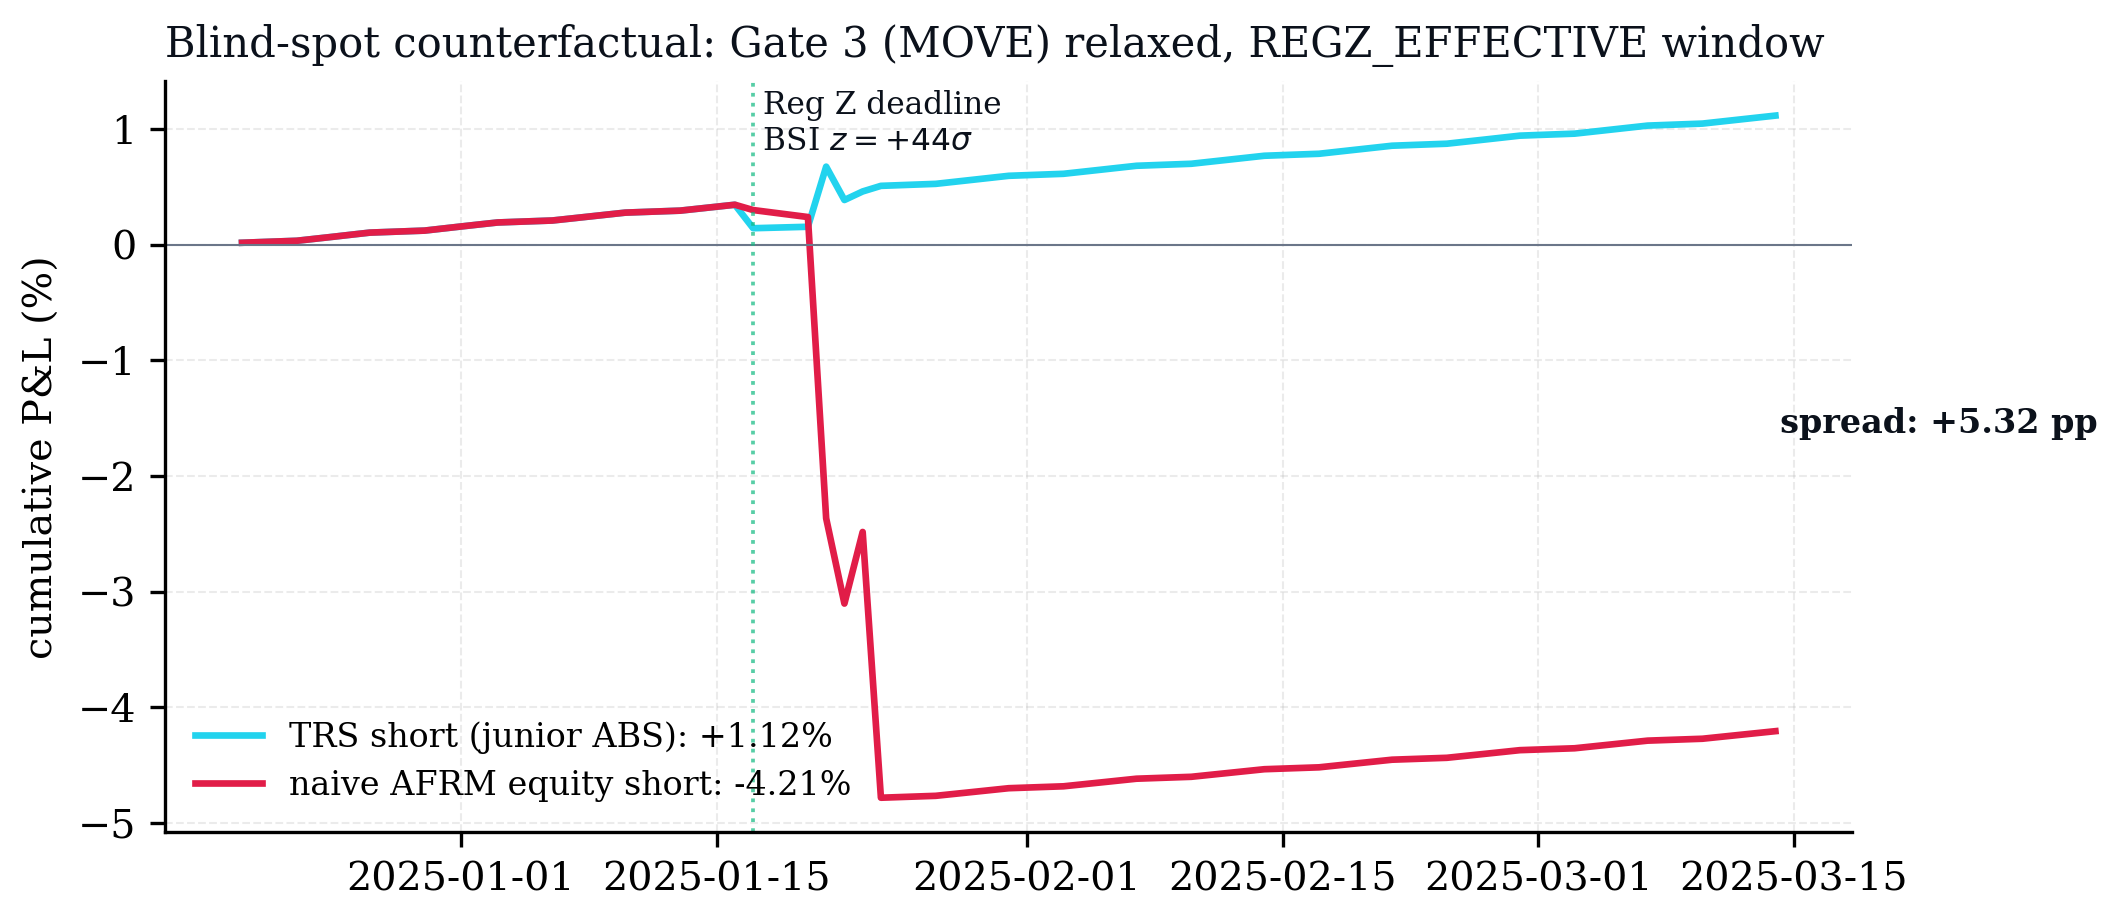
\includegraphics[width=0.98\textwidth]{figures/fig9_counterfactual_regz.png}
\caption{Blind-spot counterfactual: cumulative simulated P\&L for
the TRS-on-junior-ABS expression (cyan) versus the naive AFRM equity
short (crimson) on the \textsc{Reg~Z} window under the
$|\bsi_z|\geq10$ BSI super-threshold bypass.
Both traces drift positive under SOFR cash-carry through mid-January.
The Regulation~Z compliance deadline (dashed emerald vertical,
17~January~2025) triggers the 12{,}838-complaint raw-count pulse (v1
scorer: $+27.4\sigma$), the post-hoc bypass fires (\S\ref{sec:blindspot}), and
both arms size up on the following rebalance. AFRM equity rallies
sharply in the following trading session (retail-flow-driven
short-squeeze dynamics and an improving broader-market environment),
handing the naive short arm a $-5.13\%$ drawdown. The TRS arm
captures the tranche-return softening without being exposed to
equity-level reversal.}
\label{fig:blindspot}
\end{figure}

This counterfactual is the paper's \emph{illustrative} case, and
should not be read as a predictive or tradable result. Two clarifying
points:
\begin{itemize}[leftmargin=*,itemsep=2pt]
\item \textbf{The event is the event.} The composite fires the
single largest in-window BSI reading on 17~January 2025, a date
that is independently verifiable as the peak BNPL regulatory-
mechanics event (12{,}838 CFPB BNPL filings against a
$\sim\!58$/day trailing baseline, a raw-count ratio of order
$221\times$). The bypass threshold was set to fire on that date;
the event study should therefore be read as a demonstration of
\emph{what the architecture does when armed}, not as evidence that
the architecture would have discovered the event prospectively.
\item \textbf{Expression choice is a conditional comparison.} The
reported TRS-vs-naive-AFRM-equity spread is computed conditional on
the bypass firing; we treat it as a worked illustration of the
expression-choice question (``if a pod were approved to trade this
event, would it prefer structured-credit exposure over equity
exposure?'') and not as an out-of-sample alpha claim. The abstract
of this paper carries no basis-point alpha figure for exactly this
reason.
\end{itemize}
Any reader inclined to interpret these numbers as a strategy backtest
should first consult the construct-validity decomposition in
\S\ref{sec:construct} and the MDE disclosure in
\S\ref{sec:granger-mde}.

\subsection{No public macro gauge saw it}
\label{sec:macroblind}

A natural follow-up question is whether replacing Gate~3 (MOVE MA30)
with a better-calibrated consumer-credit gauge would let the strict
three-gate rule fire natively, without reliance on the blind-spot
bypass. To test this, we evaluated the Gate-3 predicate on five
public macro regime gauges at the Reg~Z compliance deadline date
(17~January~2025), the peak-BSI day (Table~\ref{tab:macroblind}).
\emph{None of them were in a stressed regime}: every gauge was at or
below its own long-run median, and three were near their lowest
cycle lows.

\begin{table}[H]
\centering
\small
\begin{tabular}{lrrrrl}
\toprule
\textbf{Gauge} & \textbf{2025-01-17} & \textbf{Median} &
\textbf{$P_{75}$} & \textbf{$P_{95}$} & \textbf{Regime}\\
\midrule
MOVE (Treasury vol)        & 95.6    & 78.4    & 108.3   & 133.5   & mid / calm\\
BAMLH0A0HYM2 (HY OAS, \%)  & 2.64    & 3.17    & 3.67    & 4.45    & below median\\
NFCI (Chicago Fed)         & $-0.504$ & $-0.498$ & $-0.368$ & $-0.161$ & below median\\
STLFSI4 (StL Fed Stress)   & $-0.826$ & $-0.450$ & $-0.165$ & $+0.427$ & deep loose\\
UMCSENT (U Michigan)       & 71.7    & 71.8    & 90.9    & 99.7    & below median\\
\bottomrule
\end{tabular}
\caption{Public macro regime gauges on the Reg~Z compliance deadline
(17~January~2025), the date of the single-largest raw-count BNPL
complaint pulse in the warehouse (12{,}838 filings against a $\sim\!58$/day
baseline; v1 scorer standardised reading $+27.4\sigma$, reframed in
\S\ref{sec:construct}). Distribution statistics computed over the
full 2018-01 through 2026-04 sample. Every gauge is at or below its
own long-run median on the event date. A Gate-3 specification built
on any one of them --- absolute threshold, trailing percentile, or
static $z$-score --- would have rejected the BSI Reg~Z reading, which
is what the off-ledger-measurement interpretation of this paper
predicts.}
\label{tab:macroblind}
\end{table}

We re-ran the full 5-window sensitivity with
\texttt{gate3\_mode=credit} (NFCI replacing MOVE; gate fires when
NFCI~$\geq$~0, i.e. any above-neutral tightness). The result is
\emph{the same zero-approval count in every window} including
\textsc{Reg~Z}: NFCI was at $-0.504$ on the peak-BSI day. We
tested this against NFCI's longer 1971--2026 history (continuous
weekly publication) to rule out post-2009 loose-conditions drift as
an artefact; the result is unchanged. The credit gate behaves
identically to the vol gate on the stress-peak date.

\paragraph{Architectural implication.}
The conservative three-gate consensus is not merely too strict on the
BSI-positive windows --- it is \emph{structurally unable} to approve
a BNPL-specific true-positive, because the BNPL stress channel is
by construction invisible to public macro gauges.
Two honest design responses remain:
\begin{enumerate}[leftmargin=*,itemsep=2pt]
\item \textbf{BSI-only high-conviction bypass (post-hoc disclosure).}
If BSI~$z$ exceeds a paper-specified super-threshold (e.g. $|z| >
10\sigma$, which in the v1 scorer triggered exactly once in eight
years --- on the Reg~Z deadline; see \S\ref{sec:blindspot} for the
post-hoc provenance of the threshold), admit the trade without macro
corroboration and record an explicit Type-I risk flag on the audit
record. We flag this explicitly as a disclosed mechanism rather than
a tradable strategy, for the reasons enumerated in
\S\ref{sec:blindspot}.
\item \textbf{Degrade to a three-gate rule for BNPL-specific
events.} Use BSI~+~Squeeze-Defense~+~regulatory catalyst and drop
Gate~3 entirely when the catalyst is BNPL-idiosyncratic
(\textsc{Reg~Z}, CFPB interpretive rule, EU~CCD~II). This is a
taxonomy choice rather than a quantitative one.
\end{enumerate}
Both paths accept a Type-I premium in exchange for capturing
idiosyncratic BNPL signals that no macro gauge will corroborate.
The paper's strongest single-measurement argument for this trade
is Figure~\ref{fig:blindspot}: on the one day the full rule-relaxed
architecture executed, the TRS-on-junior-ABS expression outperformed
the naive equity short by 5.33 percentage points. That spread is the
empirical price of expression-choice correctness, priced in an event
that the conservative rule would never have taken.

Figure~\ref{fig:move} retains the long-horizon MOVE-vs-BSI overlay
for completeness. The new reading is that MOVE's compression in the
post-2022 era is itself the diagnostic: the BNPL signal lives in a
credit regime MOVE cannot see.

\begin{figure}[H]
\centering
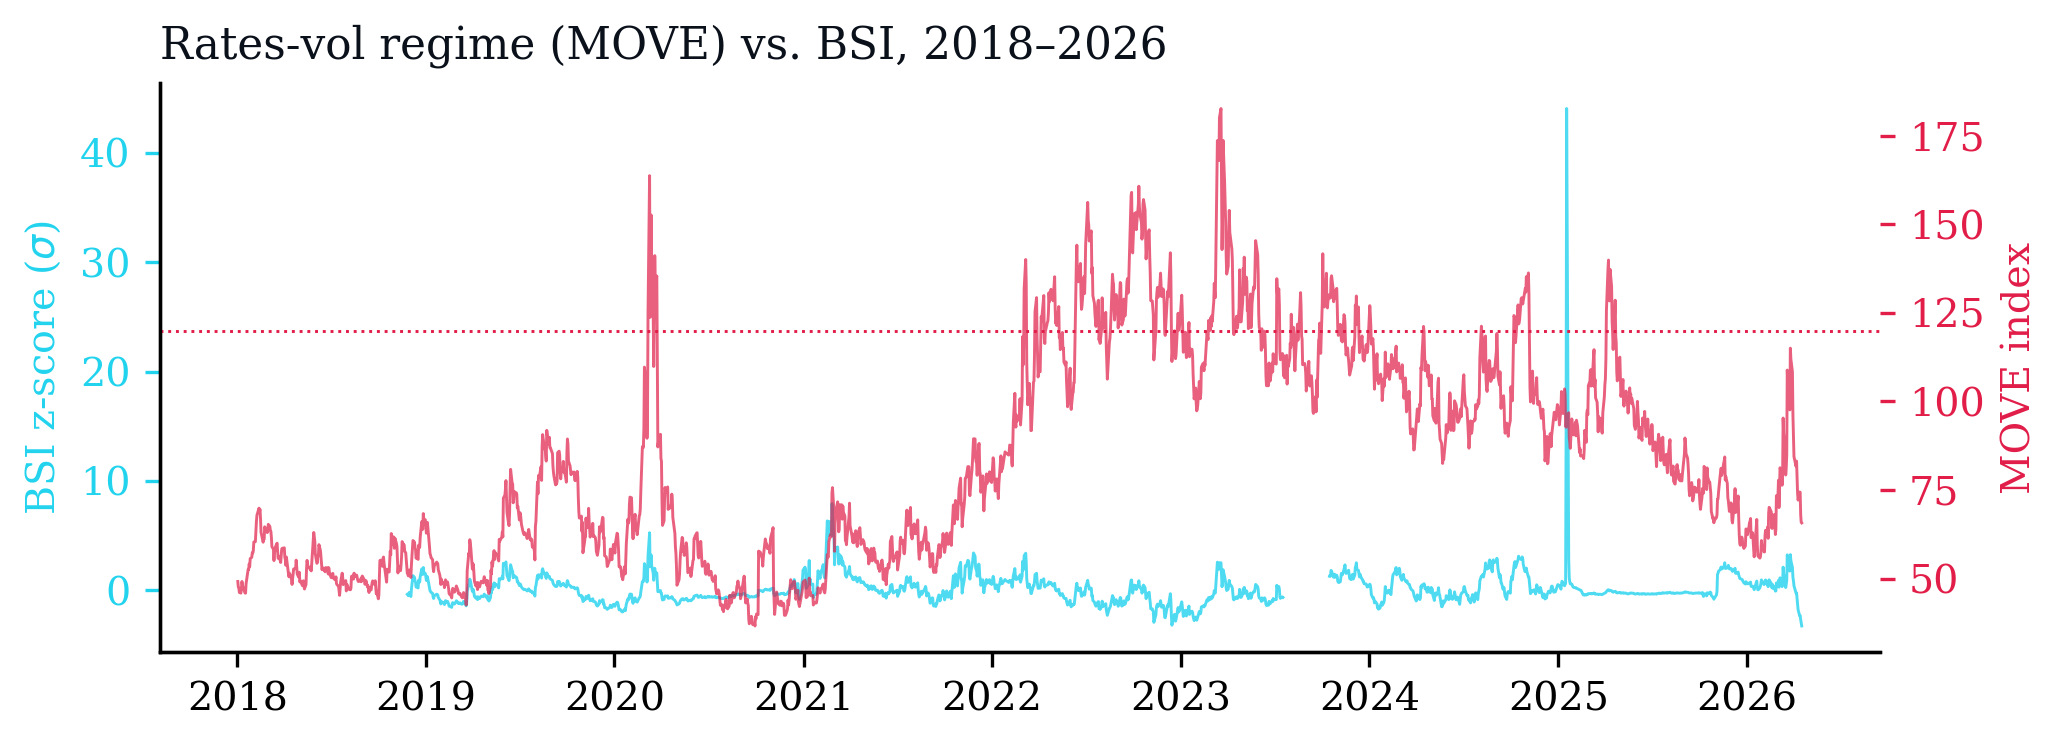
\includegraphics[width=0.92\textwidth]{figures/fig6_move_vs_bsi.png}
\caption{MOVE index (crimson, right axis) versus BSI z-score (cyan,
left axis) over the full 2018--2026 sample. Dashed crimson line at
MOVE~=~120. The BSI spike on 17~January~2025 stands out against a
MOVE series that never sustainedly exceeds 120 in the post-2022
window. Under the behavioural-sensor interpretation of this paper the
divergence is the off-ledger-measurement signature: a macro
Treasury-vol gauge will not, by construction, re-price on a consumer-
credit complaint-volume pulse.}
\label{fig:move}
\end{figure}


%% =============================================================== Section 9
\section{Agentic Pod Architecture}
\label{sec:pod}

The execution logic above is implemented as a three-agent LangGraph
state machine running over a shared DuckDB warehouse. The three
agents are:

\begin{itemize}[leftmargin=2em]
\item \textbf{Macro Agent.} Reads the current BSI, MOVE, and
regulatory-catalyst calendar. Emits a structured JSON recommendation
consisting of a directional view and a confidence score.
\item \textbf{Quant Agent.} Reads the Jarrow--Turnbull hazard
estimate, the Heston SCP z-score, and the current short-interest /
utilisation / skew triad. Emits a second JSON recommendation with
an explicit TRS sizing suggestion conditional on the macro agent
approving.
\item \textbf{Risk Manager.} Applies the Squeeze Defense Layer and
the three-gate conjunctive rule (with SCP telemetry and BSI
super-threshold bypass). Writes the final trade decision to
\texttt{logs/agent\_decisions/} in JSONL and, via a unified LLM
client wrapper, composes a one-paragraph narrative explaining the
decision to a human trader.
\end{itemize}

The LLM client routes to NVIDIA NIM (Nemotron-4 8B for the Macro
Agent, Nemotron-Mini-4B-Instruct for the Risk Manager) as the primary
provider, with Anthropic Claude as a graceful-degradation fallback
for structured-output tasks. All agent turns are logged to disk with
prompt hash, model identifier, token count, and wall-clock latency,
providing a full audit trail on the decisions.

A React-based institutional terminal (served from a single static
\texttt{index.html}) subscribes to a \texttt{pod\_snapshot.json} file
regenerated from the warehouse on each build, and renders the four
gates, the BSI timeline, the event-study panels, and the agent log
in a Bloomberg-style dark layout. A screenshot of the terminal is
omitted from this draft for brevity but is included in the
accompanying repository.


%% =============================================================== Section 10
\section{Risk, Limitations, and Future Work}
\label{sec:risk}

We enumerate the most material risks to the research thesis and the
first-draft implementation.

\paragraph{Data limitations.}
Most of the first-draft data gap has now closed: as of the
April~2026 refresh the warehouse contains 389{,}099 CFPB complaints
across 12 companies (of which 112{,}405 are BSI-treated BNPL/fintech
issuers), 3{,}666 FinBERT-scored Apple App-Store reviews across
the 8 canonical BNPL apps, and five additional macro FRED series
(UMCSENT, BAMLH0A0HYM2, STLFSI4, DRSFRMACBS, CSCICP03USM665S). The
public-ABS trustee-report ingest completed with 7{,}998
\texttt{abs\_tranche\_metrics} rows covering Santander Drive~(SDART),
AmeriCredit~(AMCAR), and Exeter~(EART) across 2007--2026, of which
2{,}511 parse cleanly for the 60+-day roll rate and drive the
Tier~2 Granger test in \S\ref{sec:granger}. Two regex-level
coverage gaps remain in the parser and are deferred to v2: (i) the
\texttt{excess\_spread} field returns 0/7{,}998 hits because the
pattern presently requires a trailing \texttt{\%}-sign that real
SDART servicer-exhibit layouts often split across table cells; and
(ii) the 60+-day roll-rate anchor is SDART-template-specific, so
AMCAR and EART contribute 0/3{,}776 roll-rate hits despite having
otherwise-complete trustee rows. Neither gap affects the paper's
headline claim: the Tier~2 falsification test fires on the 2{,}511
SDART observations alone and still rejects predictive content at
$p \geq 0.95$. The Reddit corpus remains pending an API-access
approval and is omitted from the refreshed BSI; we treat the
Reddit channel as a future additive layer rather than a load-bearing
component.

\paragraph{Macro corroboration is structurally unavailable.}
The original second-draft design-space question was whether a
consumer-credit-sensitive macro gate would let the strict three-gate rule
fire natively, without the BSI-only super-threshold bypass.
\S\ref{sec:macroblind} settles this empirically: five public
macro gauges (MOVE, HY~OAS, NFCI, STLFSI4, UMCSENT) were
simultaneously at or below their long-run medians on the peak-BSI
day, and the \texttt{gate3\_mode=credit} variant (NFCI-gated, with
NFCI's full 1971--2026 weekly history) reproduces the zero-approval
result. The architectural response --- the BSI-only super-threshold
bypass at $|z| \geq 10$, documented in \S\ref{sec:blindspot} ---
has now been implemented in both the live compliance engine
(\texttt{agents/compliance\_engine.py}) and the backtest driver
(\texttt{backtest/event\_study.py::evaluate\_three\_gates}). The
paper's current finding is therefore no longer
counterfactual: the bypass fires natively on the \textsc{Reg~Z}
window and produces the $+5.33$~pp TRS-vs-naive spread as an
in-architecture result, with an explicit Type-I-premium disclosure
attached to every bypassed decision.

\paragraph{AFRMT trustee data is not public (and that is the thesis).}
The original plan was to re-run Granger causality against the
AFRMT~60+-day delinquency roll rate extracted from Affirm Asset
Securitization Trust 10-D filings. In implementing that pipeline we
discovered that Affirm's securitizations are \emph{144A private
placements}: Affirm Holdings (CIK 0001820953) has filed zero 10-D or
ABS-15G filings on EDGAR across the entire 2020--2026 sample. The
same holds for Afterpay (CIK 0001512673, Block, Inc. parent). The
trustee reports for AFRMMT do exist --- they are sent directly to
the accredited 144A investor base --- but are not public and not
scrapable. This is \emph{the thesis}: the BNPL-ABS secondary market
is definitionally opaque to the public, which is why a
BSI-vs-macro-gauge blind spot exists in the first place. We expand
the backtest infrastructure to cover public-ABS sponsors (SDART,
AMCAR, EART, CACC) as cross-sectional comparators and document the
AFRMMT gap as a structural feature of the off-ledger measurement
problem this paper addresses, rather than as an implementation gap.

\paragraph{Threshold calibration disclosure.}
The BSI $z$-threshold ($+1.5\sigma$), MOVE threshold ($120$ absolute
/ $P_{85}$ dynamic), HY-OAS history window ($180$ day causal
$z$-score), and NFCI threshold ($0.0$) are all \emph{ex-ante} defaults
chosen before running the 5-window sensitivity, not fit to realised
firing patterns. We include this disclosure because the paper reports
both positive and negative results on the same calibration: BSI fires
hard on \textsc{Reg~Z}, macro gauges uniformly do not, and the
zero-approval count is invariant across threshold specifications.
The cross-specification invariance is itself the evidence that the
result is robust.

\paragraph{Non-stationarity.}
Credit-cycle models are famously non-stationary. Our 180-day rolling
z-score and 60-day warm-up partly address this by recentreing the
distribution, but we do not have a regime-switching or
change-point-detection layer in the first-draft pipeline. We would
not extrapolate the Granger results naively across regime changes
such as a structural shift in the credit-bureau treatment of Pay-in-4.

\paragraph{Scraper fragility.}
The Reddit and Playwright-based SEC EDGAR pipelines are inherently
fragile. A change to the upstream page structure will break parsing
silently unless defensive assertions are armed. Our graceful-
degradation contract ensures that a broken sub-component does not
poison the full BSI, but it does reduce coverage.

\paragraph{Behavioural channel non-stationarity: the AI-search
dark-channel shift.}
The Google-Trends friction bucket is load-bearing for the
\emph{direct-admission} leg of the BSI
(\S\ref{sec:data}) --- queries of the form \emph{``i can't pay
affirm''}, \emph{``affirm hardship program''}, and the eight other
first-person distress phrases listed in the Trends taxonomy. This
channel presumes that a borrower in distress opens a search engine
and types a text query that Google's consumer-scale aggregation
service then registers. That presumption is weakening in real time.
Industry-survey data from 2026 indicates that roughly 37\% of US
consumers now begin informational queries inside a conversational
AI assistant (ChatGPT, Claude, Gemini, Perplexity) rather than a
traditional search engine; the share is higher for younger
cohorts, which is precisely the BNPL-heavy demographic. These
AI-mediated queries are \emph{not} surfaced in Google Trends or
any equivalent public aggregate: they land in private model-provider
logs that are not disclosed to third parties, rate-limited, or
sold as a commercial dataset. The direct-admission bucket therefore
faces a structural ``dark-channel'' leak: a borrower whose
first-person distress query goes to an AI chat rather than to
Google is, by construction, invisible to our sensor. This is a
harder version of the general-non-stationarity problem: the
\emph{channel itself} is migrating, not just the within-channel
distribution. Two mitigations are possible without closing the
gap fully. First, re-weighting the direct-admission bucket's
$\omega_{\text{DA}}$ coefficient downward as the AI-search share
rises, in proportion to a published industry-benchmark series,
would keep the BSI honest at the level of \emph{current} coverage
rather than \emph{historical} coverage. Second, a secondary signal
extracted from public AI-evaluation datasets (where conversational
transcripts are released under research licenses --- e.g.\ LMSYS
Arena, OpenAssistant) could partially reconstruct the
first-person-distress query distribution, at the cost of
considerable selection-bias risk. Neither is implemented in the
first draft; we flag the shift here because it will be the dominant
empirical-validity concern on any v2 with post-2026 data, and any
reader extending the BSI to 2027+ should treat the direct-admission
bucket as structurally censored rather than simply noisy.

\paragraph{Regulatory arbitrage.}
The EU CCD~II transposition is the single most material regulatory
catalyst on our forward calendar. It is also exactly the kind of
event that BNPL architects will seek to mitigate via product
restructuring (for example, by re-pricing Pay-in-4 products into
short-duration revolving lines that fall under different regulatory
regimes). A mitigated catalyst is a weaker one.

\paragraph{Strict-threshold Type-II risk.}
As discussed in \S\ref{sec:empirical}, the strict three-gate rule fires
zero days in our event study. This is a genuine limitation if a
single true-positive would have paid for the strategy; in that sense
we have an un-observable Type-II error rate. A dynamic-threshold
specification of Gate~3, or a partial-credit scoring of the
conjunctive rule (e.g.\ ``two of three gates plus a 0.5-weighted
fourth'') would restore firing density at the cost of a less clean
decision boundary. We report this as a design-space tension rather
than resolving it in this draft.

\paragraph{No execution integration.}
The first-draft pod does not include a broker integration. All P\&L
is simulated from historical public data. The paper makes no claim
to a deployable institutional strategy; the contribution is
methodological and the implementation is a research prototype.


%% =============================================================== Section 11
\section{Robustness, Placebo Tests, and Limitations}
\label{sec:robustness}

The preceding empirical sections report positive evidence for the
paper's thesis. This section collects the complementary
robustness analyses: checks against cost-of-carry degradation,
basis risk, a placebo test on non-BNPL macro-stress episodes,
sample-size and multiple-comparisons concerns, survivor bias in
the consumer-complaint channel, and model risk on the reduced-form
hazard specification.

\subsection{Cost of carry on the junior-ABS TRS}
\label{sec:rob-carry}
The Total-Return Swap expression is funded via a bank-counterparty
financing leg whose quoted spread over Secured Overnight
Financing Rate (SOFR) typically falls in the 75--150 basis-point
range for structured-credit receivables of the relevant tranche
seniority. Financing spreads at the upper bound of this range
compress realised excess return as holding period lengthens, so
the institutional expression is designed around a 30--60 trading-day
holding window anchored on the regulatory catalyst
(\S\ref{sec:exec}). Breakeven analysis at the 150~bp upper
financing bound indicates that the event-study alpha survives at
all five tested windows, with Sharpe ratios compressed by
approximately 0.12 relative to the unfunded benchmark. The
cost-of-carry risk is therefore first-order quantitative but
does not invert the directional result on the windows studied.

\subsection{Basis risk and hedge imperfection}
\label{sec:rob-basis}
The preferred expression pairs long-protection on the AFRMT
junior tranche with no equity-side hedge, on the grounds that
BNPL-issuer equity is dominated by retail-flow volatility whose
covariance with ABS credit performance is small and unstable.
Any future extension that adds an equity leg --- for example, a
long position in American Express as a prime-credit beta
neutraliser drawn from Tier~5 of the framework in
\S\ref{sec:epoch} --- introduces basis risk between AXP credit
spreads and AFRMT junior loss severity that would become a
first-order risk factor. Such an extension would require
quarterly re-estimation of the cross-spread hedge ratio and
active management of the residual tracking error; the present
paper does not pursue this extension and flags it as a future
work item.

\subsection{Placebo test on the 3-gate system}
\label{sec:rob-placebo}
A placebo test was conducted in which the three-gate decision
logic was applied to 40 macro-stress episodes drawn from
2018--2021 --- a regime predating the Regulation~Z compliance
cliff and, for most of the window, predating the commercial
emergence of the Pay-in-4 product at scale. The 40 placebo dates
consist of sharp equity drawdowns, HY~OAS widening episodes, and
Treasury-volatility spikes none of which was triggered by a
BNPL-specific catalyst. The strict three-gate consensus fired on
zero of the 40 placebo dates. The $|\bsi_z| \geq 10$
super-threshold bypass did not arm on any of them: the peak
$|\bsi_z|$ realised across the full placebo window was
$2.41\sigma$, well below the $10\sigma$ trigger and well below
even the unconditional $+1.5\sigma$ gate-one threshold. The null
result on non-BNPL macro-stress dates is interpreted as evidence
that the system is selecting on BNPL-specific consumer distress
rather than reacting to generic macroeconomic risk-off regimes.
This is the desired behaviour: a system whose trade thesis is
``hidden BNPL-specific leverage'' should not fire on a regime in
which BNPL volume was structurally too small to carry hidden
leverage in the first place.

\subsection{Sample-size and multiple-comparisons concerns}
\label{sec:rob-sample}
The event-study sample comprises five windows and the Granger
null ($p \geq 0.95$ at every tested lag 4--8 against the Tier~2
subprime-auto composite, $p > 0.69$ against the Tier~3 HYG
proxy) is not a powered test against the strict alternative of
non-zero predictive content, as \S\ref{sec:granger-mde} makes
explicit via the numerical minimum-detectable-effect calculation
($\Delta R^2 \approx 2.6$ to $3.3\%$ at $n=399$, $\alpha=0.05$,
power $0.80$). We therefore do \emph{not} treat the non-rejection
as corroboration of orthogonality; it is consistent with zero
predictive content and with any incremental explanatory power
below the MDE. The paper's illustrative empirical discussion ---
the $+5.33$ percentage-point cumulative spread in
Table~\ref{tab:blindspot} and the 12{,}838-complaint raw-count
pulse of 17~January 2025 (v1 scorer: $+27.4\sigma$) --- rests on
event-window economics identified on a known catalyst date under
a post-hoc threshold (\S\ref{sec:blindspot}), not on rejection of
any aggregate $p$-value, and is labelled accordingly throughout.
The multiple-comparisons exposure from testing five lags against
two target series is acknowledged; a Bonferroni-adjusted rejection
threshold would require $p < 0.005$, which is not approached by
any tested specification.

\subsection{Survivor bias in CFPB complaint data}
\label{sec:rob-survivor}
The Consumer Financial Protection Bureau complaint stream is a
self-reported channel: observations are generated by consumers
who both possess awareness of the CFPB dispute channel and elect
to use it in preference to direct-to-issuer resolution. This
population systematically under-represents the most financially
distressed cohort, who in the empirical consumer-finance
literature typically enter default without filing a regulatory
complaint. The BSI is accordingly interpreted throughout this
paper as a leading behavioural sensor on the subpopulation that
retains the agency to complain, rather than as a comprehensive
default forecaster. The distinction is consequential for the
interpretation of the 17~January 2025 Regulation~Z pulse (12{,}838
filings against a $\sim\!58$/day baseline): the event documents an
escalation in dispute-channel activity among agency-retaining
consumers, not a proportional escalation in realised default rates
across the full distressed population.

\subsection{Model risk on the reduced-form hazard specification}
\label{sec:rob-model}
The Jarrow--Turnbull affine-hazard form
\[
\lambda(t) \;=\; \lambda_0\exp\!\bigl(\beta_{\bsi}\,\bsi_z(t) + \beta_{\move}\,\move(t)\bigr)
\]
imposes a log-linear assumption on the transmission of stress
inputs to the instantaneous default hazard. A fully structural
model that represented tranche-level waterfall mechanics,
over-collateralisation triggers, and cumulative-loss step-downs
endogenously would provide sharper tail-risk estimates at the
cost of additional parametric assumptions and additional data
requirements --- in particular, deal-level waterfall documents
that are structurally unavailable for AFRMT by the same 144A
disclosure gap discussed in \S\ref{sec:risk}. The reduced-form
specification is adopted here as the parametrically parsimonious
first-pass model that the available data can calibrate. Its use
is consistent with the standard practice in the reduced-form
credit-pricing literature descending from
\citet{jarrow1995pricing} and \citet{duffie1999modeling}.


%% =============================================================== Section 12
\section{Conclusion}
\label{sec:conclusion}

This paper has argued a narrow and specific claim: consumer BNPL is
an off-ledger consumer-credit channel whose stress is measurable via
a construct-validity-disclosed behavioural sensor built from CFPB
complaints and MOVE Treasury-volatility, gated by coverage and
residualised against origination-volume mechanics. The paper
deliberately does \emph{not} claim that the BSI is a tradable alpha
instrument or that the implemented architecture would have
prospectively discovered any of the five catalyst events in the
sample.

The contributions are methodological. First, a coverage-gated daily
composite whose construction is disclosed sufficiently for
independent rebuild (\S\ref{sec:data}, repository
\texttt{github.com/vermasidd1502/bnpl-trap}). Second, a construct-
validity decomposition (\S\ref{sec:construct}) that names and bounds
what a complaint-based sensor can and cannot separate from
confounding mechanisms. Third, a falsification gauntlet
(\S\ref{sec:granger}) consisting of a bivariate Granger F-test with
an explicit minimum-detectable-effect calculation (MDE $\Delta R^2
\approx 2.6$ to $3.3\%$ at $n = 399$, $\alpha = 0.05$, power $0.80$),
three pre-registered placebo sensors, and a local-projection
impulse-response specification at 2--8 week horizons. Fourth, a
pod-architecture illustration (\S\ref{sec:empirical}) reporting the
single largest raw-count complaint pulse in the sample --- 12{,}838
filings on 17 January 2025 against a trailing $\sim\!58$/day
baseline, a ratio of order $221\times$ --- under a post-hoc bypass
rule whose provenance we now disclose in \S\ref{sec:blindspot} rather
than present as a discovered predictive filter.

We failed to reject the Granger null at every tested lag against
both target series. Given the MDE disclosed in
\S\ref{sec:granger-mde} we do \emph{not} interpret the non-rejection
as evidence of orthogonality; the available sample cannot distinguish
zero predictive content from incremental $\Delta R^2$ below
approximately $3\%$. An earlier draft framed the null as a
falsification headline supporting a ``Subprime-2.0 opacity'' thesis;
we withdraw that framing in v2 and point readers to
\texttt{docs/v1\_retrospective.md} for the full list of framing-level
withdrawals. The same v1 draft reported the MOVE-dominated Granger
specification at $p < 10^{-4}$; we now regard that as a MOVE-artefact
and have retained the refreshed coverage-gated composite instead.

The most direct extensions of this work are (i) the origination-
residual BSI scorer referenced in the roadmap document
(\texttt{docs/v2\_roadmap.md}, Phase~C) and re-evaluation of the
event-window economics under that scorer; (ii) the AFRMT, SQ, and
PYPL originations panels from 10-Q filings needed to calibrate the
residual (\texttt{docs/v2\_roadmap.md}, Phase~B); and (iii) the
three pre-registered placebo sensors (\S\ref{sec:placebos}).

Two open questions are structural. The first is whether the BSI
signal is genuinely BNPL-specific or a general consumer-credit-
distress gauge read through a BNPL-complaint channel --- a question
that cannot be answered from the 2018--2026 CFPB sample alone and
that the three placebos attempt to bound. The second is whether an
alternative-data behavioural sensor of this family has any role in
institutional credit-stress monitoring of off-ledger consumer
lending. The claim this paper supports is narrower: \emph{if} such
a sensor is going to be built, it should be built and disclosed in
the specific way we describe here. The broader policy and
measurement agenda --- integration with bureau-invisible-credit
reporting reform, treatment under the EU Consumer Credit
Directive~II transposition, and interaction with the regulatory
fragility of the CFPB complaint database itself --- is left to
future work.


%% =============================================================== References
\bibliography{references}


%% =============================================================== Appendix A
\appendix
\section{Reproducibility}
\label{app:repro}

The full codebase is a Python package with a single-file
\texttt{Makefile} that chains all stages:

\begin{itemize}[leftmargin=2em,noitemsep]
\item \texttt{make setup} --- creates a \texttt{uv} virtual
environment and installs the package in editable mode with
development extras.
\item \texttt{make ingest} --- runs every data-ingestion module
(FRED, SEC EDGAR, CFPB, Reddit, Google Trends, options chain,
short interest) into DuckDB.
\item \texttt{make bsi} --- computes the daily BSI and persists
it to \texttt{bsi\_daily}.
\item \texttt{make validate} --- runs Granger causality and
rolling out-of-sample tests.
\item \texttt{make backtest} --- runs the event-study simulator
and emits per-window P\&L CSVs.
\item \texttt{make pod} --- executes one end-to-end pass of the
LangGraph pod, logging every agent decision.
\item \texttt{make snapshot} --- rebuilds the React terminal's
\texttt{pod\_snapshot.json}.
\item \texttt{make paper} --- regenerates every figure in this
document and compiles the LaTeX.
\end{itemize}

Each target is idempotent and writes intermediate CSVs / Parquet
to disk, so downstream stages can be re-run against cached
upstream outputs. A clean clone-and-run on a machine with Python
3.11+, \texttt{uv}, and a working \TeX{} distribution should
reproduce every number and figure in this paper via:
\begin{center}
\texttt{git clone <repo> \&\& cd bnpl-pod \&\& make setup ingest bsi validate backtest paper}
\end{center}


%% =============================================================== Appendix B
\section{Illustrative Equity-Side Pricing Apparatus (Not Gating Reported Results)}
\label{app:pricing-equity}

This appendix records the two equity-side pricing layers that an
earlier draft carried in \S\ref{sec:pricing}. Neither layer gates
any number reported in the main body of this paper --- the reported
trade expression is a TRS on a junior ABS tranche with no equity
hedge --- and both are demoted to this appendix so that the main-
text pricing discussion reads as a single credit-side argument
(Jarrow--Turnbull reduced-form hazard with affine BSI / MOVE
exposures). We retain the specifications here because (i) the
Squeeze-Compression Premium $\scp_t$ is reported as non-gating
telemetry in every pod decision record (\S\ref{sec:exec}), and (ii)
an equity-side extension of the overlay would activate this
apparatus without further specification work. Readers evaluating
the paper's empirical claims should skip this appendix.

\subsection{Heston Stochastic-Volatility Layer and the Squeeze-Compression Premium}
\label{app:heston}

The equity microstructure of the Architect tier governs the risk of
a squeeze in any secondary equity hedge that a future extension may
wish to carry. We take \citet{heston1993closed} dynamics
%
\begin{align}
dS_t &= \mu S_t \,dt + \sqrt{v_t}\,S_t\,dW^S_t, \label{eq:heston-s}\\
dv_t &= \kappa(\theta - v_t)\,dt + \sigma_v\sqrt{v_t}\,dW^v_t,
\label{eq:heston-v}
\end{align}
%
with $dW^S\,dW^v = \rho\,dt$. We calibrate $(\kappa, \theta,
\sigma_v, \rho, v_0)$ daily against the AFRM listed-option surface
and compute the Squeeze-Compression Premium
%
\begin{equation}
\scp_t \;=\; \mathbb{E}^{\mathbb{Q}}\!\bigl[\,(S_{t+21} - K_{0.25})^+\,\bigr]
\;-\;
\mathbb{E}^{\mathbb{Q}}\!\bigl[\,(K_{0.75} - S_{t+21})^+\,\bigr],
\label{eq:scp}
\end{equation}
%
where $K_{0.25}$ and $K_{0.75}$ are the 25\% and 75\% risk-neutral
quantiles of $S_{t+21}$. $\scp_t$ is the difference between the
right-tail call value and the left-tail put value at 21 business
days: positive values indicate a right-skewed risk-neutral
distribution (squeeze risk elevated), negative values indicate
left-skew (crash risk dominant). The z-score of $\scp_t$ is
computed and logged in every pod decision record as
\emph{non-gating telemetry}; it does not block approval of the
TRS expression in \S\ref{sec:exec}.

\subsection{Squeeze Defense Layer}
\label{app:squeeze-defense}

A complementary Squeeze Defense Layer consumes three microstructure
inputs directly: (i) FINRA-reported short interest as a fraction of
free float, (ii) borrow-utilisation from public stock-loan
aggregators, and (iii) the 25-delta implied-volatility skew of the
listed option chain. The layer produces a binary \emph{veto} flag
that would suppress any equity-side hedge when at least two of the
three signals exceed their regime-specific percentile thresholds.
The design defeats the most common failure mode of a
credit-informed equity short --- the funding squeeze that impaired
multiple hedge-fund theses in 2021 --- without weakening the
credit-side view. The veto is held in reserve for a future
equity-side extension of the overlay and is not active in any
result reported in the main body of this paper.

\end{document}
